\documentclass[11pt,a4paper]{article}

\usepackage[T1]{fontenc}
\usepackage[utf8]{inputenc}
\usepackage{lmodern}
\usepackage[margin=2.4cm]{geometry}
\usepackage{amsmath,amssymb,bm}
\usepackage{booktabs,array,tabularx,multirow}
\usepackage{graphicx}
\usepackage{enumitem}
\usepackage{xcolor}
\usepackage{tikz}
\usetikzlibrary{arrows.meta,decorations.pathreplacing,calc,patterns}
\usepackage[colorlinks=true,linkcolor=teal!70!black,citecolor=teal!70!black,urlcolor=teal!70!black]{hyperref}
\usepackage{caption}
\captionsetup{font=small,labelfont=bf}

\setlength{\parskip}{0.4em}
\setlength{\parindent}{0pt}
\newcommand{\nj}{\textsc{nj}}
\newcommand{\nh}{\textsc{nh}}
\newcommand{\thead}{\tau_{\mathrm{cross}}}
\newcommand{\tcross}{\tau_{\mathrm{cross}}}
\newcommand{\tpp}{\tau_{\mathrm{pp}}}
\newcommand{\tv}{\tau_{v}}
\newcommand{\lv}{\ell_{v}}
\newcommand{\vb}{v_{\mathrm{belt}}}

\title{\textbf{How Far Must the Camera See?}\\[0.3em]
\large The value of upstream visibility and pre-positioning in a shared-head conveyor cell,
across geometries and operating conditions}
\author{laser-conveyor-optimization\\\small\url{https://github.com/juanlopez-gif/laser-conveyor-optimization}}
\date{November 2026 --- draft 1.6 (results of versions 0.7.13, 0.7.21 and 0.7.28; referee corrections of 0.7.34--0.7.38; bibliographic audit of 0.7.39; scientific review of 0.7.40; closure review of 0.7.41)}

\begin{document}
\maketitle

\begin{abstract}
A single XY laser head processes parts that arrive on three parallel conveyors. The head
can only reach parts inside a working zone; a camera may also see a stretch of the entry
zone upstream of it. We ask an engineering question: how far upstream must the camera see,
and what must the controller be allowed to do with the view, for the visibility to pay
off? Three paired simulation studies answer it, each on realizations reserved for it and
used once for its prespecified analysis, with a dispatching rule as the primary controller and, in the first two, a
learned dispatching policy as a secondary one. In the \emph{reference cell} (eight regimes, 30 realizations)
we separate \emph{seeing} earlier (the same actions, a wider view) from \emph{acting}
earlier (sending the idle head towards a part before it reaches the zone): widening the
view alone produced small effects in every regime, while acting on it reduced the
penalized flow time by 2.8--7.4\,\% (network) and 2.7--7.4\,\% (rule) in the four nominal-load regimes. The \emph{geometry
bench} (72 regimes: belt spacing 6--18~cm, transverse head speed 5--15~cm/s, along-belt
head speed 5 and 10~cm/s, two loads, Poisson and bursty arrivals; 60 realizations) then
measures the gain of acting on a common grid of 0--10~s of anticipation (the visible
length divided by the belt speed: seconds of belt motion, to which any stop of that belt
adds clock time). Pre-positioning
passes the frozen benefit criterion (an estimated gain of at least 1~s per part with a
lower 95\,\% bound of at least 0.5~s per part, design thresholds fixed before the run
without an economic calibration) in 18 of the 56 distinct cells, 13 of them
with Poisson arrivals; under the conservative criterion fixed by the protocol, retaining 90\,\% of the gain,
17 of those 18 cells first meet it at a tested anticipation of 2--7.5~s, one unresolved
within the grid; in the same 18 cells, giving the controller 3.33~s of anticipation (10~cm at
3~cm/s) instead of 10~s cost a median of 0.05~s per part and at most 0.44~s per part,
the largest value observed, and retained 71--102\,\% of the estimated gain (71\,\% in
one cell). These results use the rule's arrival-time tie-break, which a camera cannot
observe. Rerun afterwards on the same realizations with the observable tie-break (the
instant of first observation), the rule passes the benefit criterion in 19 cells (13 in
common), 3.33~s cost a median of 0.04 and at most 0.44~s per part, and only 3 of the 19
cells first meet the conservative criterion before 10~s; replicated with that key on 60
fresh realizations, 14 cells pass (9 in common with those 19), 3.33~s cost a median of
0.09 and at most 0.47~s per part (individual 95\,\% interval 0.02--0.91), and 1 of the 14
cells first meets the conservative criterion before 10~s. A shorter view cost little on
average in every analysis; the certified range of 2--7.5~s belongs to the arrival-time
key, and which cells pass the benefit criterion is not stable across realizations. In the four nominal-load Poisson cells in which both along-belt speeds pass
the criterion with the arrival-time key, halving that speed multiplied the gain by
1.2--2.4 and moved the point-estimate requirement from 1.5--3.3 to 3.3--5~s. The head's transverse crossing time, the natural design reference,
is the poorest predictor family of the required anticipation among those tested
(leave-one-out error 1.5~s unscaled, 1.75~s rescaled); the mean planned duration of the pre-positioning moves the head starts is
the best of the predictors fixed before the run (1.0~s; the factor fitted on these traces
is 1.7 times the mean planned move, each episode with a move weighted equally), a
constant of 2.8~s does nearly as well (1.1~s), and the mean of the other cells with the same
along-belt head speed, a comparator computed after the run, does better than both
(0.82~s), so the trace-based predictor's advantage is small; under the observable key, on
the original realizations (19 cells), the move duration and the speed-group mean are within 0.03~s of each other (1.72 and
1.74~s). For the rule, cells with the same crossing time, the same along-belt geometry and the
same arrival realizations are identical by the model's structure. The results support specifying the camera in seconds of
anticipation for this family of cells at the belt speed tested (3~cm/s, at which seconds
and centimetres are one unit), with the cost of a shorter view measured in the
conditions where pre-positioning pays and left undetermined where the data do not
resolve it. A third study, the \emph{belt-speed bench} (3 against 5~cm/s, four cells,
60 realizations, the rule only), tests what transfers to a faster belt: at 5~cm/s, 10~cm
of coverage cost less than a margin of 0.5~s per part fixed beforehand, against the full
50~cm view, in the two configurations with the fast along-belt axis; neither slow-axis
configuration met the benefit criterion with the full view, and the paired comparison
between speeds detected a reduction in one of the two; and the comparison between
centimetres and seconds remains open.
\end{abstract}

%====================================================================
\section{Introduction}
%====================================================================
Cells in which one shared actuator serves several moving streams are common in sorting,
packaging and marking lines \cite{S01_Mattone2000,S02_Han2020,S03_Nielsen2023,S04_Schettini2023}.
The actuator reaches a bounded window of each stream; what it does with a part depends on
where the part is when the decision is taken, and what the controller can decide depends on
what it sees. Instrumentation (which stretch of the belts a camera covers) and capability
(whether the head may move towards a part before it is reachable) are design choices that
are usually fixed before the scheduling policy is written. Line parameters have been
optimized jointly with the sequence in paced assembly lines, where every part is known in
advance \cite{Sarker2001}, and the value of seeing further has been measured for an
operator's inspection range \cite{Nawijn1981}, for item-count lookahead in robot sorting
\cite{Li2026} and for the length of an upstream buffer combined with the reach of several
packing arms \cite{Ladefoged2026}; separating the value of the view from the value of the
action it enables, for a head shared by belts that stop, has not been measured to our
knowledge.
Prior work notes the dependence without quantifying it: in a packaging line the cameras
see items 5--10~s ahead and the planner is designed around that window
\cite{S04_Schettini2023}; in a batching cell a longer buffer zone improves the objective
but raises the computation beyond its budget \cite{S03_Nielsen2023}.

This paper measures the value of upstream visibility as a function of how far upstream
the camera sees, separates it from the value of the action that the visibility enables,
and asks how the answer moves when the cell's geometry and operating conditions change.
The cell (Section~\ref{sec:cell}) has one Cartesian laser head over three parallel
conveyors. A part can be processed only inside the laser zone; while it is processed its
conveyor stops, and an unprocessed part that reaches the end of the zone stops its
conveyor until the head serves it (blocking). The controller's objective is the mean flow
time of the parts plus a penalty for blocking. An overhead camera sees the laser zone and,
upstream of it, a stretch of the entry zone; the coverage corresponds to $\tv$ seconds of
uninterrupted belt motion before a part becomes reachable, the camera's
\emph{anticipation} (stops of that belt lengthen the warning in clock time,
Section~\ref{sec:anticipation}). The design question is the value
of $\tv$.

Two things change when the camera sees further. The controller \emph{sees} parts earlier,
so that it may choose better among the parts already in the zone. And, if the cell allows
it, the controller may \emph{act} earlier: send the idle head to the entry point of a belt
on which a part is approaching, so that processing starts as soon as the part enters the
zone instead of after the head's travel. The second effect has a natural time scale, the
head's travel; the pilot of this work took the head's travel time across the conveyors,
$\tcross$, as the reference for sizing the coverage. The geometry bench was designed to
test that reference, and rejects it in favour of a measured quantity.

\textbf{Contributions.}
\begin{enumerate}[nosep]
\item A paired study of one reference cell, with its protocol frozen in the repository before the run, that separates the value of
  seeing earlier (treatment B against A) from the value of acting earlier (C against B)
  and measures the gain of acting at six visible lengths, on eight regimes and 30
  reserved realizations (seeds 7000--7029, shared with the companion paper), with a dispatching rule and a learned policy
  (Sections~\ref{sec:design} and \ref{sec:reference}). Widening the view alone changed
  little; acting on it was worth 2.8--7.4\,\% of the penalized flow time for the network
  and 2.7--7.4\,\% for the rule in the four nominal-load regimes.
\item A paired geometry bench of 72 regimes, with its protocol frozen in the repository before the run, (56 distinct cells for the
  rule) on 60 reserved realizations, with a common grid of anticipation in seconds, the
  criteria for ``worth sizing'' and ``sufficient coverage'' frozen before the run
  (Sections~\ref{sec:bench} and \ref{sec:benchresults}).
\item The answer in physical units: in the 18 cells that pass the benefit criterion, 3.33~s
  of anticipation cost a median 0.05 and at most 0.44~s per part against 10~s (the
  largest value observed);
  retaining 90\,\% of the gain conservatively needs 2.0--7.5~s in 17 of the 18 cells (one
  unresolved within the grid); the along-belt head speed is a first-order factor. These
  figures use the rule's arrival-time tie-break; a retrospective rerun with the
  observable tie-break keeps the small cost of 3.33~s (median 0.04, at most 0.44~s per
  part over 19 cells) but certifies the 90\,\% criterion before 10~s in only 3 of them,
  and a replication on 60 fresh realizations with that key gives 14 cells, a median of
  0.09 and at most 0.47~s per part, and 1 early certification
  (Section~\ref{sec:tiebreak}).
\item A test of what predicts the required anticipation: the transverse crossing time is
  the worst of the candidates and, among the candidates fixed before the run, the planned
  duration of the moves the head starts the best on the 18 cells of the arrival-time key,
  with a constant close behind (the predictor's advantage is small); on the 19 cells of the
  observable key (seeds 9000--9059) the move duration and a post hoc group mean by along-belt head speed are
  within 0.03~s of each other; for the rule, cells with the same crossing time, the same along-belt
  geometry and motion settings and the same arrival realizations are identical by
  the model's structure (Section~\ref{sec:predict}).
\item A trace-based reading of the mechanism: at the nominal load the aggregate gain per
  pre-positioning move is compatible with the saving being transmitted to the parts
  queued behind it; at the high load the queue count does not explain the size of the
  effect and the alternative (a cascade of belt stops avoided) remains a hypothesis. And
  a check, in the reference geometry, that lengthening the physical entry zone changes the
  installation's flow time while no difference in the camera's value was detected (Sections~\ref{sec:mechanism} and \ref{sec:entry}).
\end{enumerate}

The companion paper (Paper~1) presents the learned policy used here and its comparison with
search-based controllers; this paper uses it only as a secondary controller and does not
depend on its training.

%====================================================================
\section{Related work}\label{sec:related}
%====================================================================
Five strands of work touch the cell studied here. In one of them, three studies ask how
much a controller gains from seeing further ahead, each in a different setting from ours;
none separates the value of the view from the value of the action it enables.

\textbf{Lookahead and upstream information.} At a conveyor-serviced production station
with Poisson arrivals, an operator who has just finished a unit inspects a range of the
belt measured in time units and takes the first unit that arrives in it; the optimal range
depends on the number of units in a reserve, the operator's sight is assumed to cover every
range, units that pass are lost and the belt never stops \cite{Nawijn1981}. A robot arm that
takes the foremost item of one of several infeed queues, with the next $L$ items of each
queue identified, is within about 1\,\% of its full-information optimum on average already
at $L=1$ when it
votes over sampled completions of the hidden queues, while a myopic dynamic program needs
$L=20$ \cite{Li2026}: lookahead is counted in item identities, and the robot cannot act on
an item before it is at the pick point. In robotic food packing, a buffer belt ahead of
four arms with exclusive zones sets how early item weights are known; a longer buffer
reduces the overfill with diminishing returns and increases the items lost at the end of
the belt, and its value interacts with the reach given to each arm \cite{Ladefoged2026}.
Their formulation includes the time an arm needs to intercept an item, pack it and reach
the next one, but the reported simulations assume instantaneous movements and tray swaps,
so moving an arm ahead of an item is not studied; the belts run at constant speed and never
stop, and the effects are fitted by regression on dimensionless parameters. Our study
varies the physical length the camera covers and, separately, the permission to send a
shared head towards a part before it is reachable, on belts that stop, and estimates both
effects on paired realizations with criteria fixed before the run. The horizon of a
look-ahead controller is a different quantity: the 20--80~s rollout horizons tuned in
\cite{Righettini2025}, or the 30~s window of the scenario search of the companion paper,
truncate simulated futures, while the anticipation measured here is what the camera
physically observes now.

\textbf{Picking and sorting from moving conveyors.} With one arm over one belt and
Poisson arrivals, \cite{S02_Han2020} sequence the reachable objects by dynamic
programming and show by example that greedy rules (first-in, nearest-first) are not
optimal in general, with first-in best at low arrival rates and worst at high ones; the
belt never stops and objects that leave the reachable window are lost. Sorting on a
moving belt \cite{S01_Mattone2000} and value-aware sorting with availability windows
\cite{S05_Kokkalis2026} share that setting. With several arms, \cite{S03_Nielsen2023}
batch items from an infeed belt into tray lanes with a goal program solved per tray
inside a 1.8~s decision budget, and note that a longer buffer zone improves the objective
but raises the computation beyond the budget; \cite{S04_Schettini2023} schedule
identical robots along input and output conveyors by row generation and local search,
with cameras that see items 5--10~s ahead and items not picked lost at the end of the
belt. In all of these the belt never stops because of the processing and an unserved
item leaves the system; in our cell processing stops the part's belt and an unprocessed
part blocks it, so the trajectories of the remaining parts depend on the schedule, and
the visibility horizon is a parameter of the setting rather than a quantity whose value
is measured. Conveyor stops caused by unfinished work are classical in mixed-model
assembly lines \cite{Xiaobo2000,Tamura2011}, but there the launch sequence is fixed offline
and nothing is sensed; the companion paper discusses them.

\textbf{Interception of moving targets.} The moving-target travelling salesman problem
\cite{S06_Helvig2003}, its discrete- and continuous-time formulations with visibility
windows \cite{S07_Stieber2022} and the mixed-integer conic formulation over a graph of
convex sets \cite{S08_Philip2024} give exact models of a single agent intercepting
targets that move with exogenous, constant velocities, offline. The formulation behind
this paper (the project's formulation document) uses the same interception geometry
with endogenous motion: a belt's odometer stops while its part is processed or blocked.

\textbf{Blocking in conveyor systems.} Blocking as a schedule-dependent loss appears in
packaging machines whose devices obstruct each other along one infeed
\cite{S10_Briskorn2025} and in a food warehouse where full crane buffers stop the
upstream conveyors, with the blocked time minimised offline by simulation-based
metaheuristics \cite{S11_SalviaHornos2026}. Our objective charges both the blocking
events and their duration, inside the dispatching problem.

\textbf{Learned dispatching.} The learned policy used as the secondary controller
belongs to the family of dispatching policies trained from search or from expert
schedules: rollout \cite{M02_Bertsekas1997}, policy-gradient dispatching with
objective-aligned rewards \cite{S19_Zhang2020,S21_Sun2023}, offline learning from
constraint-programming schedules \cite{S20_VanRemmerden2025}, action masking
\cite{M04_Huang2022,S18_Wei2024}, and learned control of conveyor-fed robotic cells
\cite{S15_Zisgen2025,S16_Drijver2023,S17_Drakaki2017,S12_Wang2004,S13_Li2020}. Its
design and training are the subject of Paper~1; here it matters only that it uses every
observable part, so that it can turn a wider view into different decisions, which the
dispatching rule with the arrival-time tie-break cannot (with the observable tie-break the
view can change only how the rule breaks ties).

What these works leave open, and this paper measures, is how the value of the sensing
reach depends on what the controller may do with it, and how that value moves with the
geometry and the load of the cell, on paired realizations.

%====================================================================
\section{The cell and its information model}\label{sec:cell}
%====================================================================

This section describes the cell studied, its objective, the information model with the two things a camera enables, seeing a part earlier and acting on the view, and the quantities the coverage is measured against: the anticipation, the crossing time and the moves the head makes.

\subsection{Geometry and dynamics}
Figure~\ref{fig:cell} shows the cell. Parts travel in the $+x$ direction on $N=3$
conveyors at $y_k=(k-1)\,d$, $d$ the belt spacing, at a common belt speed $\vb$. The belt
has an entry zone $[0,a)$ that the head cannot reach, a laser zone $[a,b]$ of 35~cm, and
an exit zone of 10~cm. The head moves in the rectangle $[a,b]\times[0,2d]$ with
simultaneous axes at speeds $v_x$ and $v_y$, so that the travel between two points takes
$\max(\Delta x/v_x,\Delta y/v_y)$. Processing a part takes a constant $p$ seconds, during
which the part's conveyor stops. A part that reaches $b$ unprocessed stops its conveyor
until the head serves it; every such event is a \emph{blocking} event. The \emph{reference
cell} has $d=12$~cm, an entry zone of 10~cm, $\vb=3$~cm/s, $v_x=v_y=10$~cm/s, $p=2.5$~s
and mean inter-arrival times of 10, 12 and 14~s on the three belts (processing load
$\rho_p=0.64$); its heavy variant has $\vb=5$~cm/s, $v_x=v_y=5$~cm/s, $p=3$~s and
inter-arrivals of 8, 10 and 12~s ($\rho_p=0.93$, overloaded once the head's travel is
counted). The geometry bench of Section~\ref{sec:bench} varies $d$, $v_y$, $v_x$ and the
arrival rates with the other quantities fixed, and lengthens the entry zone to 35~cm so
that long anticipations can be tested. The formal model (belt odometer, exact
continuous-time constraints, time-indexed MILP) is given in the project's formulation
document and is not repeated here.

\begin{figure}[t]
\centering
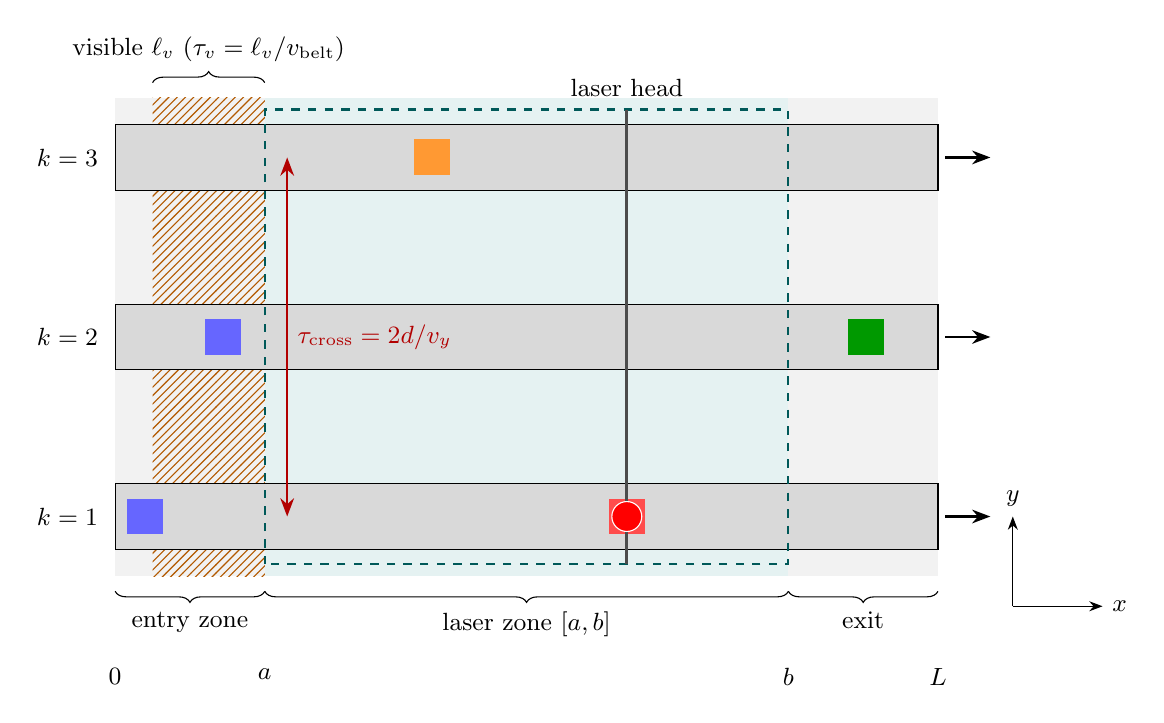
\begin{tikzpicture}[x=0.19cm,y=0.19cm,>=Stealth]
  \fill[gray!10] (0,-4) rectangle (10,28);
  \fill[teal!10] (10,-4) rectangle (45,28);
  \fill[gray!10] (45,-4) rectangle (55,28);
  \fill[pattern=north east lines,pattern color=orange!70!black] (2.5,-4) rectangle (10,28);
  \foreach \y/\n in {0/1,12/2,24/3}{
    \draw[fill=gray!30] (0,\y-2.2) rectangle (55,\y+2.2);
    \node[left] at (-0.5,\y) {\small $k=\n$};
    \draw[->,thick] (55.5,\y) -- (58.5,\y);
  }
  \draw[teal!70!black,dashed,thick] (10,-3.2) rectangle (45,27.2);
  \fill[blue!60] (0.8,-1.2) rectangle (3.2,1.2);
  \fill[blue!60] (6,10.8) rectangle (8.4,13.2);
  \fill[orange!80] (20,22.8) rectangle (22.4,25.2);
  \fill[red!70] (33,-1.2) rectangle (35.4,1.2);
  \fill[green!60!black] (49,10.8) rectangle (51.4,13.2);
  \draw[very thick,gray!60!black] (34.2,-3.2) -- (34.2,27.2);
  \draw[fill=red,draw=white] (34.2,0) circle (1.0);
  \node[above] at (34.2,27.4) {\small laser head};
  \draw[<->,thick,red!70!black] (11.5,0) -- (11.5,24) node[midway,right] {\small $\tcross=2d/v_y$};
  \draw[decorate,decoration={brace,mirror,amplitude=4pt}] (0,-5) -- (10,-5)
       node[midway,below=4pt] {\small entry zone};
  \draw[decorate,decoration={brace,amplitude=4pt}] (2.5,29) -- (10,29)
       node[midway,above=4pt] {\small visible $\lv$ ($\tv=\lv/\vb$)};
  \draw[decorate,decoration={brace,mirror,amplitude=4pt}] (10,-5) -- (45,-5)
       node[midway,below=4pt] {\small laser zone $[a,b]$};
  \draw[decorate,decoration={brace,mirror,amplitude=4pt}] (45,-5) -- (55,-5)
       node[midway,below=4pt] {\small exit};
  \node[below] at (0,-9.5) {\small $0$};
  \node[below] at (10,-9.5) {\small $a$};
  \node[below] at (45,-9.5) {\small $b$};
  \node[below] at (55,-9.5) {\small $L$};
  \draw[->] (60,-6) -- (66,-6) node[right] {\small $x$};
  \draw[->] (60,-6) -- (60,0) node[above] {\small $y$};
\end{tikzpicture}
\caption{Cell layout (top view, reference cell). Parts travel in $+x$; the head reaches
$[a,b]\times[0,2d]$. The camera sees the laser zone and the hatched stretch $[a-\lv,a)$
of the entry zone: the coverage corresponds to $\tv=\lv/\vb$ seconds of uninterrupted
belt motion before a part becomes reachable. The part on belt~1 is upstream of the visible stretch and is not seen.
$\tcross$ is the head's travel time across the conveyors.}
\label{fig:cell}
\end{figure}

\subsection{Objective}
An episode generates arrivals for 300~s and then runs until every part has left. The
objective is the \emph{penalized flow time}
\begin{equation}
J=\frac{1}{n}\sum_{j=1}^{n}(C_j-r_j)+\frac{\lambda_N N_B+\lambda_T T_B}{n},
\end{equation}
the mean flow time from arrival $r_j$ to completion $C_j$ plus a penalty for the $N_B$
blocking events and the $T_B$ conveyor-seconds stopped by blocking, with $\lambda_N=10$~s
per event and $\lambda_T=1$~s per conveyor-second. The weights are placeholders in
equivalent seconds; the economic translation of the results is left for a later version
(Section~\ref{sec:limits}). Every gain reported below is a difference of $J$ between two
configurations on the same realization; in the geometry bench it is given in seconds per
part, and it turns out to be 82--96\,\% flow time. That share makes flow time the dominant
component of the gains; it does not make threshold decisions insensitive to the weights:
with the unpenalized flow time instead of $J$, the benefit criterion of the geometry bench
(Section~\ref{sec:bench}) would pass 15 cells instead of 18 (a sensitivity computed after
the run from the released extract; the three cells lost are $d/v_y/v_x=6/15/10$~cm,
cm/s, cm/s at the high load with bursts and at the nominal load with Poisson arrivals,
and $12/15/5$ at the nominal load with bursts). In those three cells the flow-time part of
the full-view gain is 0.92, 0.86 and 0.93~s per part, below the threshold of 1~s, while the
weighted blocking events add $-0.00$, 0.08 and 0.03~s and the weighted blocked time 0.12,
0.09 and 0.08~s, bringing the totals to 1.03, 1.03 and 1.04~s (paired 95\,\% half-widths:
flow 0.47, 0.19 and 0.39; totals 0.51, 0.26 and 0.46~s per part; in the first cell the
flow-only lower limit, 0.44~s, is also below the 0.5~s of the screen): the penalty terms
decide whether these cells reach the threshold.

\subsection{Information model and pre-positioning}
A policy may use only what the cell observes. At a dispatch event (the head is free and at
least one candidate exists; the companion paper calls a dispatch event with at least two
candidates a decision epoch) the controller knows the time, the head's position and state,
the state of every belt, and, for every \emph{observable} part, its belt, position,
processing time and the instant from which it has been observed. Three observation levels
are compared:
\begin{description}[nosep]
\item[\texttt{zone}] parts inside the laser zone only (a cell without camera);
\item[\texttt{belts}] the above plus the parts in the visible stretch $[a-\lv,a)$ of the
  entry zone, with their positions ($\lv=0$ coincides with \texttt{zone});
\item[\texttt{full}] the above with the whole entry zone plus the parts waiting upstream
  of the belt entry, which the real camera cannot see (the richest input tried: an upper
  bound on the information available, not on the value a fixed controller realizes from it).
\end{description}
Under \texttt{belts} a part upstream of the visible stretch, or waiting in the hidden
queue, is unknown to the controller: it produces no observation, it is not a candidate, and
its earlier history leaves no trace once it appears. The controller knows the mean arrival
rates of the belts and the arrival horizon, but never the future arrival instants.

The head's \emph{pre-positioning} option decides what it may do with a visible part that
is still in the entry zone. With \texttt{none} the candidates are the parts already in
the laser zone; with \texttt{when\_idle}, if no part is in the zone, the head may be sent
towards a visible entry-zone part: it moves to the point $(a,y_k)$ and waits there, and
the commitment is revoked (at no cost) the moment another part is ready in the zone while
the target is still in the entry zone, so that the policy decides again; if the target itself enters the zone, alone or together with other
parts, the commitment stands. Physically, \texttt{when\_idle} needs the camera to cover the entry
zone and the head to be able to move to a point and wait; it is the design mode of the
cell. The treatments of the reference-cell study combine the two options:
\begin{center}
\begin{tabularx}{\linewidth}{@{}l l l X@{}}
\toprule
treatment & observation & pre-positioning & what it measures\\
\midrule
A & \texttt{zone} & \texttt{none} & no camera: local visibility, local actions\\
B & \texttt{belts}, $\lv=10$ & \texttt{none} & the camera: upstream visibility, the same actions\\
C & \texttt{belts}, $\lv=10$ & \texttt{when\_idle} & the camera and the action it enables\\
D & \texttt{full} & \texttt{none} & B plus the hidden queue (upper bound)\\
\midrule
$\mathrm{L}\lv/\mathrm{none}$ & \texttt{belts}, $\lv$ & \texttt{none} & coverage grid at visible length $\lv$\\
$\mathrm{L}\lv/\mathrm{when\_idle}$ & \texttt{belts}, $\lv$ & \texttt{when\_idle} & idem with pre-positioning\\
\bottomrule
\end{tabularx}
\end{center}
B against A is the value of seeing with the same actions; C against B the value of acting
on the same view; D against B the value of what the camera cannot see. The coverage grid
gives, at each $\lv$, the gain of pre-positioning \emph{with} against \emph{without} it at
the same length; this contrast, written $G(\tv)$ in seconds per part, is the quantity of
the geometry bench.

\subsection{Anticipation, crossing time and the moves the head makes}\label{sec:anticipation}
A part at $x=a-\lv$ enters the laser zone after $\tv=\lv/\vb$ seconds of belt motion:
$\tv$ is the \emph{anticipation} the camera gives, 3.33~s for the whole 10~cm entry zone of
the reference cell. It is the warning time while the belt runs; if the belt stops while the
part crosses the visible stretch (because a part of the same belt is processed or blocks),
the elapsed time from first detection to zone entry is $\tv$ plus that stopped time (10~cm
at 3~cm/s with one 2.5~s service in between: 5.83~s). All coverages in this paper are
nominal anticipations in this sense. When the head is idle at $(X,y)$ and a part is announced on belt $k$, the
pre-positioned head reaches the meeting point $(a,y_k)$ after
$\max(|X-a|/v_x,\,|y-y_k|/v_y)$ seconds. The lane component is at most the head's
travel time across the conveyors, $\tcross=2d/v_y$ (2.4~s in the reference cell); the
along-belt component is at most $35/v_x$ (3.5~s at $v_x=10$~cm/s) and small when the
head finished its previous part near the entry, as it does after a pre-positioned one.
If $\tv$ covers the move, the head is in place when the part enters; otherwise part of
the move is still paid after the part is reachable. The pilot of this work took
$\tcross$ as the reference against which the coverage curve is read, on the hypothesis
that the gain of pre-positioning grows with $\tv$ up to about $\tcross$ and levels off
beyond it. The geometry bench records, for every pre-positioning move the head starts, both
components of the planned travel at the moment the move is decided (a move may still be
revoked when another part becomes ready while its target is still upstream; revocations
are counted apart and are rare, at most
0.6 per episode in the cells analysed below), and tests $\tcross$ against the mean planned
duration of those moves, $\tpp$, as predictors of the anticipation the camera needs.

%====================================================================
\section{Experimental design}\label{sec:design}
%====================================================================

Three paired studies share the checks of this section: the reference-cell study of Section~\ref{sec:reference}, and the geometry bench and the belt-speed bench of Section~\ref{sec:benchresults}. All three evaluate \nj; the reference and geometry studies also evaluate the frozen network. Each study's protocol was fixed before its run, on realizations reserved for it and used once; for the belt-speed bench the margin and the design were proposed in the protocol, and the final choices of seed range, margin and controller are recorded with the results. The reference-cell realizations (seeds 7000--7029) are the phase-4 realizations that the companion paper analyzes for different research questions. The geometry bench's realizations were reused once more, after its run, for the retrospective rerun of Section~\ref{sec:tiebreak}, and the bench was then replicated with the observable tie-break on 60 fresh realizations (seeds 43700--43759), with the seed range, the cells, the benefit screen, the grid and the criteria fixed before that run.

\subsection{Controllers}
Two distinct implementations run every configuration of the first two studies (the
belt-speed bench runs the rule only), so that the value of information is not tied to one
policy; they are not independent, since the network descends from a training chain whose
expert searched over the rule, so their agreement on shared realizations is evidence of
robustness to the choice of controller with shared sources of variation:
\begin{itemize}[nosep]
\item \nj\ (\texttt{nearest\_job}), the primary controller: the dispatching rule that
  chooses the candidate with the smallest interception time (ties: earliest arrival in
  the reference study and the geometry bench; since version 0.7.26 of the project the
  instant from which the part has been observable, the convention of the belt-speed
  bench, Section~\ref{sec:beltdesign}). It
  never uses a part it cannot select, so under the earliest-arrival key the
  pure-information contrasts of \nj\ (B vs A, D vs B) are zero by construction, checked
  on the geometry extract (identical \texttt{none} costs across visible lengths in every
  cell and realization), and only the action contrast (C vs B) and the coverage curve
  are informative; under the observable key the tie-break itself depends on the
  coverage, and Section~\ref{sec:belt} reports that change of the baseline; it is also geometry-agnostic, which makes it the clean
  instrument of the geometry bench. \nh\ (\texttt{nearest\_head}), the same rule restricted
  to the most downstream candidate of each belt, is also run in the reference cell.
\item the \emph{network}, the secondary controller: the learned dispatching policy of
  Paper~1, a Transformer over tokens of the observable parts, the belts, the head and the
  cell parameters, trained by expert iteration from a sampled-future search teacher on a
  family of cells that includes the reference regimes, with the three information levels
  in its training mix (\texttt{belts} 70\,\%, \texttt{zone} 15\,\%, \texttt{full} 15\,\%
  of the episodes). It uses every observable part, so it can turn upstream visibility into
  better choices among the zone parts (B vs A) and use the hidden queue (D vs B). A second
  network of the same size (the \emph{reference network}: the checkpoint from which the
  frozen network's training was continued, trained before bursty arrivals and slow heads
  entered the training mix) is used in Section~\ref{sec:robust} to check that the
  reference-cell contrasts survive that retraining; the two are not independent runs. In
  the geometry bench the 35~cm entry zone and the slowest along-belt speed with the fastest
  lane speed lie at or beyond the network's training ranges, so its results there also
  measure that extrapolation. The network's decision latency is 8--12~ms per decision
  (median, one thread, machine fully loaded).
\end{itemize}

\subsection{The reference-cell study}\label{sec:refdesign}
Eight regimes cross the load (nominal, heavy), the arrival process (Poisson; bursts: an
on/off Poisson source with the same mean rate, on 30\,\% of the time in on-periods of mean
20~s) and the head speed (nominal; slow: $v_x,v_y$ halved). Table~\ref{tab:regimes} gives
the physical scales of each regime: the belt speed, the head speed, $\tcross$, the
anticipation of the whole entry zone, and the level of the \nj\ rule in treatment~B, which
is the common baseline of its tables. The heavy regimes are overloaded by design: the
head has almost no idle time, and they bound the results from the other side. Every
regime runs the treatments A--D and the coverage grid $\lv\in\{0,1,2.5,5,7.5,10\}$~cm
with \texttt{none} and \texttt{when\_idle}.

\begin{table}[t]
\centering\small
\caption{Reference-cell regimes and physical scales. $\tcross$ is the head's travel time
across the conveyors; the entry zone is given in seconds of belt travel; parts, penalized
flow time, blocking events and blocked conveyor-seconds are means per episode for \nj\ in
B over the 30 realizations (seeds 7000--7029, shared with the companion paper).}
\label{tab:regimes}
\resizebox{\linewidth}{!}{% generated by experiments/paper2_figures.py from data/phase4_info.csv
\begin{tabular}{@{}lccccrrrr@{}}
\toprule
regime & belt [cm/s] & head [cm/s] & $\tau_{\mathrm{cross}}$ [s] & entry zone [s] & parts & \textsc{nj} in B [s/part] & blocking events & blocked [conv.\,s] \\
\midrule
real / Poisson / nominal head & 3 & 10 & 2.4 & 3.33 & 78 & 21.8 & 7.8 & 122 \\
real / Poisson / slow head & 3 & 5 & 4.8 & 3.33 & 78 & 42.1 & 14.8 & 322 \\
real / bursts / nominal head & 3 & 10 & 2.4 & 3.33 & 73 & 27.6 & 5.1 & 93 \\
real / bursts / slow head & 3 & 5 & 4.8 & 3.33 & 73 & 41.3 & 8.2 & 184 \\
heavy / Poisson / nominal head & 5 & 5 & 4.8 & 2.00 & 94 & 73.5 & 18.2 & 601 \\
heavy / Poisson / slow head & 5 & 2.5 & 9.6 & 2.00 & 94 & 104.0 & 14.2 & 720 \\
heavy / bursts / nominal head & 5 & 5 & 4.8 & 2.00 & 89 & 72.0 & 11.1 & 399 \\
heavy / bursts / slow head & 5 & 2.5 & 9.6 & 2.00 & 89 & 93.6 & 9.1 & 508 \\
\bottomrule
\end{tabular}
}
\end{table}

Every configuration of a regime runs on the same 30 realizations (common random numbers:
the same arrival instants and processing times), so that every contrast is a paired
difference per realization. For a contrast written ``X vs Y'' we report
\[
\Delta=100\,\Bigl(\frac{1}{30}\sum_{\omega}\frac{J_X(\omega)}{J_Y(\omega)}-1\Bigr)\ [\%],
\]
the mean over the realizations $\omega$ of the paired cost ratio, with a normal 95\,\%
confidence interval, and in parentheses the number of realizations in which
$J_X(\omega)<J_Y(\omega)$. A negative $\Delta$ favours $X$, the first-named
configuration. Pilots on development realizations (seeds 2000--2029, also used to choose
the network) shaped the hypotheses; the confirmatory run used 30 realizations reserved for
it (seeds 7000--7029), never seen by any design decision of this study, and run once for
its prespecified analysis with the protocol frozen beforehand (the companion paper
analyzes the same realizations for other questions).

\subsection{The geometry bench}\label{sec:bench}
The bench varies the cell around the reference cell with the belt speed (3~cm/s), the
processing time (2.5~s), the laser and exit zones and the penalties fixed:
\begin{itemize}[nosep]
\item \textbf{belt spacing} $d\in\{6,12,18\}$~cm and \textbf{transverse head speed}
  $v_y\in\{5,10,15\}$~cm/s, nine combinations with
  $\tcross=2d/v_y\in\{0.8,1.2,1.6,2.4,2.4,2.4,3.6,4.8,7.2\}$~s;
\item \textbf{along-belt head speed} $v_x\in\{5,10\}$~cm/s;
\item \textbf{load}, by the arrival rates only: nominal (mean inter-arrivals 10, 12, 14~s;
  $\rho_p=0.64$) and high (7, 8.5, 10~s; $\rho_p=0.90$);
\item \textbf{arrivals}: Poisson, or the bursty source of the reference study at the same
  mean rate per belt.
\end{itemize}
That is 72 regimes. The entry zone is 35~cm in every cell, long enough for the largest
anticipation of the grid; the laser zone, the workspace and the head's home move with it.
The \textbf{coverage grid is common in seconds}: $\tv\in\{0,0.5,1,1.5,2,2.5,3.33,5,7.5,
10\}$~s, i.e.\ $\lv=3\tv\in\{0,1.5,\dots,30\}$~cm, each with \texttt{none} and
\texttt{when\_idle}. Every configuration runs on the same \textbf{60 realizations}
(seeds 9000--9059, reserved for this bench and used once for its prespecified analysis;
reused for the retrospective rerun of Section~\ref{sec:tiebreak}). A \textbf{physical-length
check} runs the reference geometry with its original 10~cm entry at the grid points up to
10~cm, against the 35~cm entry at the same points, to separate the effect of the longer
installation from the camera's reach. The bench was preceded by a pilot on development
realizations (seeds 3000--3029, nine geometries, $v_x=10$, nominal load), whose findings
shaped the bench: the pilot's crossing-time grid was replaced by the common grid in
seconds, $v_x$ was added as a factor, and the trace statistics were added.

\textbf{Measures and criteria, frozen before the run.}
\begin{itemize}[nosep]
\item \emph{Primary:} $G(\tv)=J_{\mathrm{none}}(\tv)-J_{\mathrm{when\_idle}}(\tv)$ in
  seconds of penalized flow time per part, paired, with a 95\,\% interval; positive means
  that pre-positioning helps. The unpenalized flow, the blocking events and the blocked
  belt-seconds are reported with it.
\item \emph{Cost of less coverage:} $J_{\mathrm{when\_idle}}(\tv)-J_{\mathrm{when\_idle}}(10\,\mathrm{s})$
  at $\tv=1.5$, 2.5 and 3.33~s, paired: what the cell loses, already pre-positioning, by
  seeing less.
\item \emph{Worth sizing:} a regime is worth sizing the coverage for when
  $G(10\,\mathrm{s})\ge1$~s per part and its lower 95\,\% bound is $\ge0.5$~s per part.
  Both thresholds are design decisions fixed before the run, without an economic
  calibration; the 0.5~s per part here is the lower bound required of the benefit, a
  different use of the number from the margin of Section~\ref{sec:beltdesign}.
  Otherwise the absolute effect is reported and the sufficient coverage is left
  \emph{undetermined} for that regime.
\item \emph{Sufficient coverage (knee):} the first grid anticipation $\tau$ whose paired
  contrast $G(\tau)-0.9\,G(10\,\mathrm{s})$ is $\ge0$ (point estimate) and, conservatively,
  whose lower simultaneous 95\,\% bound is $\ge0$ with a Bonferroni factor over the nine
  non-zero grid points ($z=2.773$). The conservative value is the headline. The knee is the
  \emph{first} tested point that meets the contrast; later points are not required to meet
  it too, and the simultaneous adjustment is within each cell, not across cells.
\item \emph{Predictors of the knee} (rule, regimes worth sizing): the Spearman rank
  correlation of the knee with $\tcross$ and with $\tpp$ (the mean of the planned
  $\max(t_x,t_y)$ over the pre-positioning moves started at 10~s of anticipation), and the leave-one-out mean
  absolute error of four models: knee $=\tcross$, knee $=a\,\tcross$, knee $=b\,\tpp$,
  knee $=$ constant. The lowest error is the paper's answer to ``what predicts the
  coverage''.
\item \emph{Mechanism:} the number of unfinished parts in the system is recorded at each
  pre-positioning move; the aggregate gain per move divided by that number should be of
  the order of the move's duration (within a factor of two) if the saving of a move is
  transmitted to the parts queued behind it.
\item \emph{Network only:} $J_{\mathrm{when\_idle}}(0)-J_{\mathrm{when\_idle}}(\tv)$ (the
  value of widening the view with the network's mode input fixed) and
  $J_{\mathrm{none}}(0)-J_{\mathrm{none}}(\tv)$ (the value of seeing with the same actions),
  reported apart.
\end{itemize}
The protocol, the hypotheses of the pilot and the results are recorded in the project's
methods documentation, written before and after the run respectively.

\subsection{The belt-speed bench}\label{sec:beltdesign}
Every cell of the geometry bench runs its belts at 3~cm/s, so within it seconds of
anticipation and centimetres of visible belt are one variable ($\lv=3\tv$). A third
bench, with its hypotheses, margin and criteria written before the run, asks what
transfers to a faster belt: at 5~cm/s the same 10~cm give 2.00~s of anticipation and
3.33~s need 16.7~cm. It runs the belt at 3 and at 5~cm/s on four cells of the geometry
bench, $d=12$~cm, $v_y=10$~cm/s ($\tcross=2.4$~s) and $d=6$~cm, $v_y=15$~cm/s
($\tcross=0.8$~s), each with $v_x=5$ and $10$~cm/s, all four passing the benefit
criterion at 3~cm/s in Section~\ref{sec:benchresults}; nominal load, Poisson arrivals,
a common physical entry zone of 50~cm (10~s of free transit at 5~cm/s), a common grid of
twelve visible lengths in centimetres (0--50~cm, including 10, 15 and 16.7~cm, with
five pairs of lengths giving the same anticipation at the two speeds), \texttt{none}
against \texttt{when\_idle} at every length, \nj\ as the only controller, and the same
arrival realizations at both speeds (the arrival streams are seeded per belt and do not
depend on the belt speed), so that differences between speeds are paired as well; 60
realizations on a new reserved range (seeds 10000--10059), used once. The decision is taken per cell on the
paired cost of the shorter view against the full 50~cm view at 5~cm/s,
$C_5(\ell)=J_{\mathrm{when\_idle},5}(\ell)-J_{\mathrm{when\_idle},5}(50\,\mathrm{cm})$,
with a margin $\delta=0.5$~s per part fixed before the run (the largest cost of 3.33~s
observed in the 18 useful cells of the geometry bench was 0.44; a design decision, the
largest loss admitted when shortening the view, distinct from the 0.5~s per part lower
bound of the benefit criterion): $H_{\mathrm{cm}}$, 10~cm
keep the benefit ($C_5(10\,\mathrm{cm})\le\delta$); $H_{\mathrm{s}}$, 10~cm do not but
16.7~cm do; $H_{\mathrm{neither}}$, 16.7~cm do not either. A cell that passes the
benefit criterion at 3~cm/s and fails it at 5~cm/s is reported as ``benefit lost at this
speed'' and the question is moot for it. The conservative reading uses the 95\,\% bound
of the cost against $\delta$ (the headline), the point reading the estimate. It was
written beforehand that the two cells with $v_x=10$~cm/s answer $H_{\mathrm{cm}}$
under either hypothesis, on the expectation that their requirement at 3~cm/s is at most
2~s, so that only the two cells with $v_x=5$~cm/s can separate the scales. That expectation
was not borne out in full: in the geometry bench (35~cm entry, nominal load, Poisson
arrivals) their conservative requirements are 2.0~s ($d/v_y=6/15$) and 3.33~s ($12/10$)
with the arrival-time key, 7.5~s each with the observable key on the same realizations,
and 2~s and 10~s with the observable key on fresh realizations (Tables~\ref{tab:sufficient},
\ref{tab:tiebreak} and \ref{tab:fresh}).

\subsection{Checks}
Five checks support the causal reading. (i) \emph{Masks are respected}: unit tests change
the parts that a treatment cannot see and verify that neither the network's inputs nor the
look-ahead costs of the search policies change; in the bench every decision of every
episode is additionally checked at run time (no candidate upstream of the visible stretch
in 179\,520 episodes; these run-time assertions are recorded as totals). The extracts of
(v) support the cost comparisons by seed, including the equality of the two modes at
zero coverage for the rule and the identity of (iv); exact arrival histories and the mask
checks require the simulator's records, not the rows (a row carries the seed and the
number of parts, in the belt-speed bench also the sum of the arrival instants).
(ii) \emph{Simulator}: every run uses an exact event-driven
simulator of the cell; on the reference realizations, for the two rules \nj\ and \nh\ in
both modes, the fixed-step reference engine at a
1~ms step gives the identical processing order in 96\,\% of the episodes and a mean
absolute difference of $J$ of 0.03--0.06\,\% (the network was not run on that engine). (iii) \emph{Schedules} are checked against
the formal model's constraints. (iv) \emph{Structure}: with simultaneous axes the belts'
$y$ coordinates enter the simulator only through the lane travel times $d/v_y$ and the
head's home, so two cells with the same $\tcross$ and the same $x$ geometry must give
identical costs for the rule, realization by realization; the bench contains three such
cells ($d/v_y=6/5$, $12/10$, $18/15$~cm per cm/s) and the prediction holds exactly
(maximum difference $2.6\cdot10^{-13}$~s over 2\,400 paired episodes in each of the eight
$v_x\times$load$\times$arrivals blocks). The rule's bench therefore has 56 distinct cells,
and the predictor analysis counts the triplet once. (v) \emph{Reproducibility}: the
per-episode results of the three confirmatory runs are distributed with the source
(\texttt{data/phase4\_info.csv}, 15\,360 episodes; \texttt{data/geometry\_bench.csv.gz},
179\,520 episodes; \texttt{data/belt\_speed\_bench.csv.gz}, 11\,520 episodes) together with
the scripts that generate the figures and tables of those runs; the analysis of the
bench extracts needs only NumPy and Matplotlib. The retrospective rerun of
Section~\ref{sec:tiebreak} is distributed as its aggregate output
(\texttt{data/recheck\_0\_7\_39\_geometry.txt}), with the paired intervals of its
shortening costs in \texttt{data/closure\_0\_7\_40/observable\_short\_cost\_ci.txt}, and the
replication on fresh realizations as per-episode results
(\texttt{data/closure\_0\_7\_40/paper2\_prospective\_episodes.csv.gz}, 20\,160 episodes).
Tables~\ref{tab:tiebreak} and \ref{tab:fresh} are generated from these files by a
script, \texttt{paper2\_\allowbreak closure\_\allowbreak tables.py}, in
\texttt{experiments/closure\_0\_7\_40}; Table~\ref{tab:cohorts}
is entered by hand from the same outputs.

%====================================================================
\section{The reference cell: seeing against acting}\label{sec:reference}
%====================================================================

The reference-cell study separates seeing from acting on the eight regimes of one cell, then measures the coverage curve of that cell and checks the robustness of the contrasts to the controller.

\subsection{Widening the view alone changes little; acting on it is worth 3--7\,\%}\label{sec:seeing}
Table~\ref{tab:contrasts} and Figure~\ref{fig:contrasts} give the contrasts between
treatments.

\begin{table}[t]
\centering\small
\caption{Reference cell: contrasts between treatments (paired $\Delta$ of the penalized
flow time, \%, 95\,\% CI; in parentheses the realizations, out of 30, in which the
first-named treatment is cheaper; bold: the interval excludes zero). For \nj\ the
contrasts B vs A and D vs B are zero by construction (arrival-time tie-break). Seeds
7000--7029, shared with the companion paper.}
\label{tab:contrasts}
\resizebox{\linewidth}{!}{% generated by experiments/paper2_figures.py from results/experiments/phase4/bench.json
\begin{tabular}{@{}lcccc|c@{}}
\toprule
 & \multicolumn{4}{c|}{network} & \textsc{nj} \\
regime & B vs A & C vs B & D vs B & C vs A & C vs B \\
\midrule
real / Poisson / nominal head & $+0.85 \pm 1.14$ (11/30) & {\boldmath$-7.37 \pm 1.87$} (27/30) & $-0.32 \pm 0.78$ (12/30) & {\boldmath$-6.63 \pm 1.87$} (27/30) & {\boldmath$-7.37 \pm 2.49$} (27/30) \\
real / Poisson / slow head & $-0.89 \pm 1.24$ (19/30) & {\boldmath$-3.56 \pm 2.48$} (22/30) & $+0.03 \pm 0.99$ (12/30) & {\boldmath$-4.51 \pm 2.23$} (25/30) & {\boldmath$-3.61 \pm 2.55$} (22/30) \\
real / bursts / nominal head & $+0.71 \pm 1.16$ (10/30) & {\boldmath$-2.75 \pm 1.50$} (24/30) & $-0.74 \pm 1.05$ (12/30) & {\boldmath$-2.12 \pm 1.46$} (22/30) & {\boldmath$-2.71 \pm 1.72$} (23/30) \\
real / bursts / slow head & $-0.03 \pm 1.06$ (9/30) & {\boldmath$-4.26 \pm 2.19$} (24/30) & $+0.24 \pm 1.00$ (12/30) & {\boldmath$-4.32 \pm 2.28$} (25/30) & {\boldmath$-3.88 \pm 2.26$} (25/30) \\
heavy / Poisson / nominal head & $-0.63 \pm 1.08$ (17/30) & $-1.27 \pm 1.34$ (22/30) & {\boldmath$-2.66 \pm 1.43$} (23/30) & {\boldmath$-1.95 \pm 1.19$} (23/30) & $+0.09 \pm 1.16$ (19/30) \\
heavy / Poisson / slow head & $-1.34 \pm 1.66$ (15/30) & $-0.01 \pm 1.98$ (16/30) & {\boldmath$-3.74 \pm 1.87$} (20/30) & $-1.43 \pm 2.09$ (19/30) & $+0.46 \pm 2.31$ (12/30) \\
heavy / bursts / nominal head & $-0.42 \pm 0.63$ (15/30) & {\boldmath$-1.60 \pm 1.14$} (22/30) & $-0.42 \pm 0.77$ (14/30) & {\boldmath$-2.03 \pm 1.05$} (24/30) & $-0.33 \pm 1.38$ (19/30) \\
heavy / bursts / slow head & {\boldmath$-1.31 \pm 0.74$} (15/30) & $+0.64 \pm 1.16$ (15/30) & $+0.04 \pm 0.85$ (9/30) & $-0.67 \pm 1.51$ (19/30) & $+1.22 \pm 2.11$ (16/30) \\
\bottomrule
\end{tabular}
}
\end{table}

\begin{figure}[t]
\centering
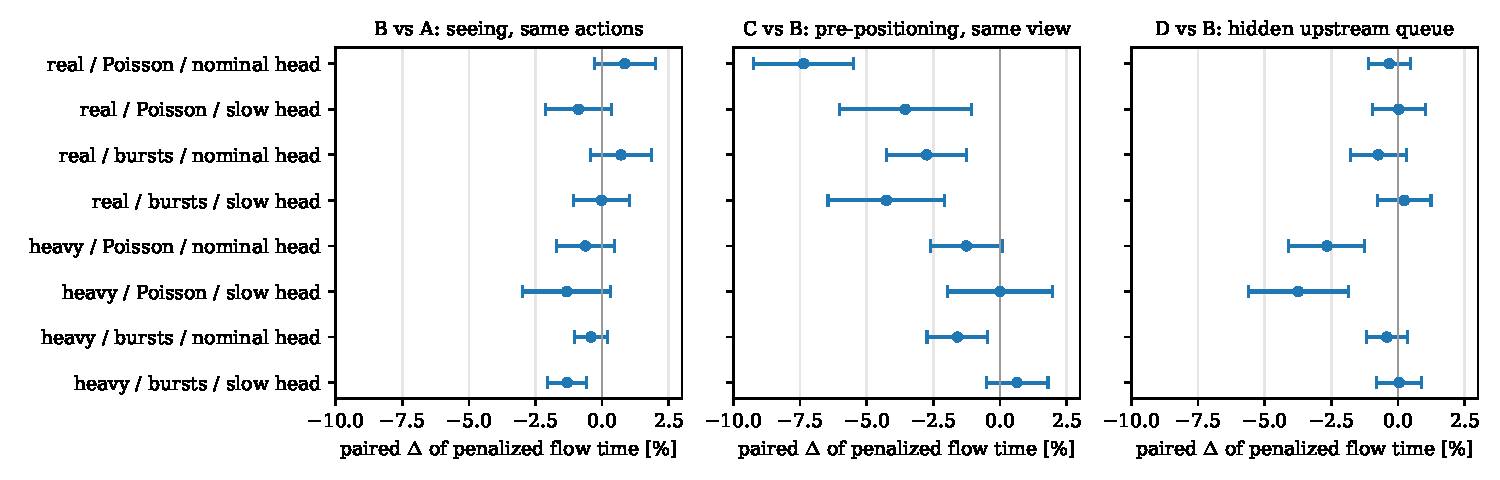
\includegraphics[width=\linewidth]{figures/contrasts.pdf}
\caption{Reference cell: the network's contrasts between treatments on the eight regimes
(paired $\Delta$ of the penalized flow time, 95\,\% CI; negative favours the first-named
treatment; filled markers: the interval excludes zero). Seeds 7000--7029, shared with the companion paper.}
\label{fig:contrasts}
\end{figure}

\textbf{B vs A.} With the same actions, seeing the entry zone produced small effects in
every regime tested. For the network the contrast lies between $-1.3$ and $+0.9$\,\%
with intervals of $\pm0.6$ to $\pm1.7$. One cell favours the wider view by a modest but
significant margin: the heavy load with bursts and a slow head ($-1.31\pm0.74$, the
regime with the longest lane travel relative to the processing); the seven other
intervals include zero. The network does use the upstream parts, since its inputs change
with them and its level in A differs from its level in B by up to 1.5 points in either
direction, but outside that regime the use does not translate into a better schedule.
Under treatment~B the controller can only choose among the parts already in the zone, and
it must choose one whenever there is one: a dispatch event has a non-empty candidate set,
and waiting for a part that is about to enter is not an action. Upstream visibility can
therefore help it only through the order of the zone parts; in this cell that is worth
little, since processing takes 2.5~s and the head crosses the lanes in 2.4~s, so a part
that enters the zone during a processing is reachable soon after it ends whatever the
order.

\textbf{C vs B.} Acting on the same view is where the value is, in the four nominal-load
regimes, where the head has idle time. At the nominal load the network gains $7.4\pm1.9$\,\% with the nominal head,
$3.6\pm2.5$\,\% with the slow head, $2.8\pm1.5$\,\% with bursts and $4.3\pm2.2$\,\% with
both, in 22--27 of the 30 realizations; the \nj\ rule gains the same ($7.4$, $3.6$, $2.7$,
$3.9$\,\%). In absolute terms, at the nominal regime the rule's penalized flow time falls
from 21.8 to 20.3~s per part (its mean flow time from 19.3 to 18.0~s); the blocking
penalty barely moves, so the gain is flow time, i.e.\ the head's travel removed from the
parts' waiting. At the heavy load the head is seldom idle and the contrast is within
$\pm1.3$ points (significant only with bursts and the nominal head, $-1.6\pm1.1$). Bursts
and a slower head both reduce the value of acting early (from 7.4 to 2.8 and 3.6 points)
and neither creates a value of seeing early: with bursts the parts of a burst arrive
together and only the first of them finds the head free; with a slow head the travel to
pre-position is longer than the anticipation the zone offers.

\textbf{D vs B.} What the camera cannot see, the parts waiting upstream of the belt entry,
is worth $2.7\pm1.4$\,\% (nominal head) and $3.7\pm1.9$\,\% (slow head) for the network at
the heavy load with Poisson arrivals, in 20--23 of the 30 realizations, and is within
$\pm1$ point in the six other regimes. At the heavy load the belts queue upstream most of
the time and knowing how many parts wait behind each belt lets the controller choose
which belt to relieve; at the nominal load the hidden queue is usually empty. This is the
one regime of the reference study in which seeing the hidden queue (D vs B), as opposed
to more capability, had value, and it is the information the camera's length cannot
provide; seeing more belt with the same actions (B vs A) had a small detected value in
one regime only, the heavy load with bursts and a slow head (Section~\ref{sec:robust}). The network saw the \texttt{full} level in 15\,\% of its training episodes; its use of
the queue is that of a controller trained mostly without it.

\subsection{The coverage curve of the reference cell}\label{sec:coverage}
Figure~\ref{fig:coverage} and Table~\ref{tab:coverage} give, at each visible length, the
gain of pre-positioning with against without it at that same length. For the reference
cell the lengths 1, 2.5, 5, 7.5 and 10~cm are 0.33, 0.83, 1.67, 2.50 and 3.33~s of
anticipation, against $\tcross=2.4$~s (nominal head) or 4.8~s (slow head).

\begin{figure}[t]
\centering
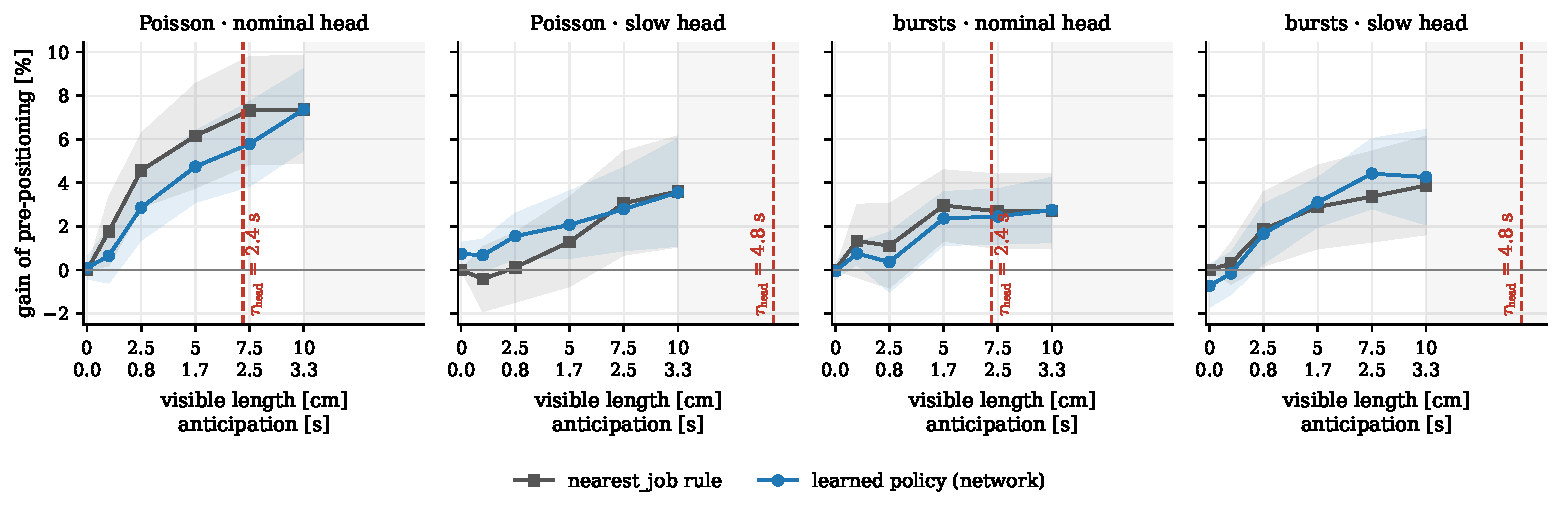
\includegraphics[width=\linewidth]{figures/coverage_real.pdf}
\caption{Reference cell, nominal load: reduction of the penalized flow time obtained by
pre-positioning (\texttt{when\_idle} against \texttt{none} at the same visible length,
paired; bands are 95\,\% CIs) against the visible length and the anticipation
$\tv=\lv/\vb$. The dashed line is the head's travel time across the conveyors,
$\tcross$; the shaded area lies beyond the entry zone. Seeds 7000--7029, shared with the companion paper.}
\label{fig:coverage}
\end{figure}

\begin{table}[t]
\centering\small
\caption{Reference cell, nominal load: gain of pre-positioning at each visible length
(\texttt{when\_idle} vs \texttt{none}, same length; paired $\Delta$ of the penalized flow
time, \%, 95\,\% CI) and, in parentheses, its share of the gain with the whole entry zone
(10~cm). The second header row gives the anticipation in seconds at the belt speed of
3~cm/s. Seeds 7000--7029, shared with the companion paper.}
\label{tab:coverage}
\resizebox{\linewidth}{!}{% generated by experiments/paper2_figures.py from data/phase4_info.csv
\begin{tabular}{@{}llcccccc@{}}
\toprule
regime & policy & $\tau_{\mathrm{head}}$ & 1 cm & 2.5 cm & 5 cm & 7.5 cm & 10 cm \\
 & & [s] & 0.33 s & 0.83 s & 1.67 s & 2.50 s & 3.33 s \\
\midrule
real / Poisson / nominal head & \textsc{nj} & 2.4 & $-1.76 \pm 1.58$ (24\,\%) & $-4.57 \pm 1.71$ (62\,\%) & $-6.16 \pm 2.40$ (84\,\%) & $-7.32 \pm 2.48$ (99\,\%) & $-7.37 \pm 2.49$ (100\,\%) \\
 & network &  & $-0.65 \pm 1.25$ (9\,\%) & $-2.86 \pm 1.50$ (39\,\%) & $-4.74 \pm 1.64$ (64\,\%) & $-5.78 \pm 1.95$ (78\,\%) & $-7.37 \pm 1.87$ (100\,\%) \\
real / Poisson / slow head & \textsc{nj} & 4.8 & $+0.42 \pm 1.50$ (-12\,\%) & $-0.12 \pm 1.60$ (3\,\%) & $-1.29 \pm 2.06$ (36\,\%) & $-3.06 \pm 2.38$ (85\,\%) & $-3.61 \pm 2.55$ (100\,\%) \\
 & network &  & $-0.68 \pm 0.74$ (19\,\%) & $-1.55 \pm 1.06$ (44\,\%) & $-2.08 \pm 1.55$ (58\,\%) & $-2.79 \pm 1.91$ (78\,\%) & $-3.56 \pm 2.48$ (100\,\%) \\
real / bursts / nominal head & \textsc{nj} & 2.4 & $-1.33 \pm 1.68$ (49\,\%) & $-1.11 \pm 1.94$ (41\,\%) & $-2.96 \pm 1.64$ (109\,\%) & $-2.69 \pm 1.71$ (99\,\%) & $-2.71 \pm 1.72$ (100\,\%) \\
 & network &  & $-0.76 \pm 0.50$ (27\,\%) & $-0.36 \pm 1.38$ (13\,\%) & $-2.36 \pm 1.24$ (86\,\%) & $-2.46 \pm 1.27$ (89\,\%) & $-2.75 \pm 1.50$ (100\,\%) \\
real / bursts / slow head & \textsc{nj} & 4.8 & $-0.30 \pm 0.95$ (8\,\%) & $-1.87 \pm 1.71$ (48\,\%) & $-2.89 \pm 1.92$ (74\,\%) & $-3.37 \pm 2.09$ (87\,\%) & $-3.88 \pm 2.26$ (100\,\%) \\
 & network &  & $+0.16 \pm 0.97$ (-4\,\%) & $-1.66 \pm 1.36$ (39\,\%) & $-3.10 \pm 1.14$ (73\,\%) & $-4.42 \pm 1.61$ (104\,\%) & $-4.26 \pm 2.19$ (100\,\%) \\
\bottomrule
\end{tabular}
}
\end{table}

With the nominal head and Poisson arrivals the rule's gain grows almost linearly with the
anticipation (24, 62 and 84\,\% of the whole-zone gain at 0.33, 0.83 and 1.67~s) and is
complete at 2.5~s (99\,\%), the first grid point beyond $\tcross$; the network's curve also
rises with the anticipation, with lower shares and a later knee (9, 39, 64, 78\,\%; 16, 53, 81 and 97\,\% when its
\texttt{none} baseline is pooled over the lengths, a sensitivity analysis that moves the
share by 15--20 points because the network's \texttt{none} level varies with $\lv$ by up
to 1.3 points). With a head twice as slow the curve does not saturate inside the entry
zone (the rule gains 36\,\% at 1.67~s and 85\,\% at 2.5~s; the network 58 and 78\,\%). The
share answers how much of the benefit a shorter view retains; the designer's question is
how much worse the cell is, already pre-positioning, with a shorter view
(Table~\ref{tab:direct}): at the nominal regime, 7.5~cm instead of 10~cm costs
$+0.24\pm0.57$\,\% for the network and $+0.05\pm0.04$\,\% for the rule, against
$+1.33\pm0.91$ and $+1.36\pm0.86$\,\% with 5~cm; with the slow head 7.5~cm costs
$1.4\pm1.1$ and $0.7\pm1.8$\,\%, and 5~cm $2.2\pm1.5$ and $2.7\pm2.3$\,\%. The two
readings differ for the network because its \texttt{none} level at 7.5~cm is $1.4\pm1.0$
points below its level at 10~cm, which the share counts as benefit lost and the direct
contrast does not carry.

\begin{table}[t]
\centering\small
\caption{Reference cell: two answers to ``is a shorter view enough?'' Left: cost of
pre-positioning with 5 or 7.5~cm against with the whole 10~cm zone (\texttt{when\_idle}
at both lengths; paired $\Delta$ of the penalized flow time, \%, 95\,\% CI; positive = the
shorter view costs more; in parentheses, realizations in which the shorter view was
better). Right: pre-positioning benefit lost, the gain of Table~\ref{tab:coverage} at
the shorter length minus the gain at 10~cm, per realization (points). A secondary
analysis of the phase-4 data, added after the run. Bold: the
interval excludes zero. Seeds 7000--7029, shared with the companion paper.}
\label{tab:direct}
\resizebox{\linewidth}{!}{% generated by experiments/paper2_figures.py from data/phase4_info.csv
\begin{tabular}{@{}llcccc@{}}
\toprule
regime & policy & \multicolumn{2}{c}{5 cm against 10 cm} & \multicolumn{2}{c}{7.5 cm against 10 cm} \\
 & & cost [\%] & benefit lost [pts] & cost [\%] & benefit lost [pts] \\
\midrule
real / Poisson / nominal head & \textsc{nj} & {\boldmath$+1.36 \pm 0.86$} (2/30) & {\boldmath$+1.21 \pm 0.78$} & {\boldmath$+0.05 \pm 0.04$} (0/30) & {\boldmath$+0.05 \pm 0.04$} \\
 & network & {\boldmath$+1.33 \pm 0.91$} (5/30) & {\boldmath$+2.63 \pm 1.04$} & $+0.24 \pm 0.57$ (5/30) & {\boldmath$+1.59 \pm 1.08$} \\
real / Poisson / slow head & \textsc{nj} & {\boldmath$+2.70 \pm 2.32$} (8/30) & {\boldmath$+2.32 \pm 2.19$} & $+0.73 \pm 1.82$ (6/30) & $+0.55 \pm 1.78$ \\
 & network & {\boldmath$+2.23 \pm 1.46$} (5/30) & $+1.48 \pm 1.88$ & {\boldmath$+1.36 \pm 1.11$} (3/30) & $+0.77 \pm 1.51$ \\
real / bursts / nominal head & \textsc{nj} & $-0.22 \pm 0.67$ (4/30) & $-0.24 \pm 0.70$ & $+0.03 \pm 0.04$ (0/30) & $+0.03 \pm 0.04$ \\
 & network & $+0.34 \pm 0.55$ (5/30) & $+0.39 \pm 0.94$ & $+0.29 \pm 0.42$ (1/30) & $+0.30 \pm 0.94$ \\
real / bursts / slow head & \textsc{nj} & $+1.21 \pm 1.72$ (7/30) & $+0.99 \pm 1.64$ & $+0.59 \pm 0.80$ (2/30) & $+0.51 \pm 0.74$ \\
 & network & $+1.60 \pm 1.97$ (6/30) & $+1.16 \pm 1.85$ & $+0.19 \pm 1.48$ (6/30) & $-0.16 \pm 1.56$ \\
\midrule
heavy / Poisson / nominal head & \textsc{nj} & $+0.24 \pm 0.84$ (6/30) & $+0.22 \pm 0.82$ & $+0.43 \pm 0.93$ (4/30) & $+0.40 \pm 0.92$ \\
 & network & $+0.29 \pm 0.96$ (9/30) & $+0.50 \pm 1.25$ & $-0.60 \pm 1.09$ (9/30) & $-0.21 \pm 1.32$ \\
heavy / Poisson / slow head & \textsc{nj} & $+0.29 \pm 1.82$ (16/30) & $+0.19 \pm 1.83$ & $+0.35 \pm 1.52$ (17/30) & $+0.24 \pm 1.46$ \\
 & network & $+0.50 \pm 1.98$ (16/30) & $+0.71 \pm 2.25$ & $+0.11 \pm 1.51$ (19/30) & $+0.17 \pm 1.54$ \\
heavy / bursts / nominal head & \textsc{nj} & $-0.24 \pm 1.24$ (12/30) & $-0.31 \pm 1.24$ & $+0.24 \pm 0.70$ (7/30) & $+0.22 \pm 0.71$ \\
 & network & $+0.83 \pm 0.95$ (6/30) & {\boldmath$+1.01 \pm 0.92$} & $+0.03 \pm 0.59$ (9/30) & $-0.05 \pm 0.69$ \\
heavy / bursts / slow head & \textsc{nj} & $+1.29 \pm 1.75$ (12/30) & $+1.16 \pm 1.90$ & $+0.93 \pm 1.55$ (13/30) & $+0.83 \pm 1.65$ \\
 & network & $+0.78 \pm 1.45$ (11/30) & $+0.52 \pm 1.30$ & $+0.42 \pm 1.16$ (12/30) & $+0.51 \pm 1.10$ \\
\bottomrule
\end{tabular}
}
\end{table}

Read against $\tcross$, this curve suggested that the head's travel time across the
conveyors, in seconds of belt travel, is the reference for sizing the coverage: 7.2~cm
of belt for the nominal head, between the 5~cm point (64--84\,\% of the gain) and the
7.5~cm point (78--99\,\%), and 14.4~cm for a head twice as slow, beyond the entry zone.
That reading, formed on one geometry, is the hypothesis the geometry bench was built to
test; Section~\ref{sec:predict} shows that it does not survive a change of geometry, and
why.

\subsection{Robustness to the controller}\label{sec:robust}
Table~\ref{tab:robust} repeats the three contrasts with the reference network, the
checkpoint from which the frozen network was retrained with bursts and slow heads in the
training mix; it is a check against that retraining, not against an independent run.
The comparison that respects the pairing is the difference, realization by realization,
between the two networks' contrasts (frozen minus reference): its mean is within 1 point
in 18 of the 24 cells and within 0.5 in 12, its largest value is 2.1 points (B vs A at
the heavy load with Poisson arrivals and a slow head, $-2.1\pm2.9$), and its interval
excludes zero in two cells, both C vs B, in which the frozen network obtains more from
pre-positioning ($-0.92\pm0.87$ points at the nominal regime with Poisson arrivals and
$-1.30\pm1.05$ at the heavy load with bursts and the nominal head). These are 24
exploratory comparisons with individual 95\,\% intervals, close to the one or two
exclusions of zero that chance alone would give. Both checkpoints showed a small B-vs-A
benefit in the heavy, bursty, slow-head regime ($-1.31\pm0.74$ and $-0.79\pm0.66$\,\%);
the other B-vs-A intervals of the frozen network include zero. The pattern of the
contrasts (B vs A, the value of acting at the nominal load, the value of the hidden queue at the
heavy load, the sign of every significant cell) is conserved after the retraining, with
differences of magnitude in some regimes; the reference network's coverage curve at the
nominal regime retains 76\,\% of the whole-zone gain at 5~cm and 97\,\% at 7.5~cm.

\begin{table}[t]
\centering\small
\caption{Reference cell, robustness (a secondary analysis of the phase-4 data, added after the run): the reference network's contrasts (as
Table~\ref{tab:contrasts}) and the paired difference between the frozen and the
reference network's contrasts (frozen minus reference, per realization, points; negative
= the frozen network obtains more from the treatment). Bold: the interval excludes zero. Seeds 7000--7029, shared with the companion paper.}
\label{tab:robust}
\resizebox{\linewidth}{!}{% generated by experiments/paper2_figures.py from results/experiments/phase4/bench.json
\begin{tabular}{@{}lccc|cc@{}}
\toprule
 & \multicolumn{3}{c|}{reference network} & \multicolumn{2}{c}{frozen vs reference} \\
regime & B vs A & C vs B & D vs B & in B & in C \\
\midrule
real / Poisson / nominal head & $+0.86 \pm 1.40$ (13/30) & {\boldmath$-6.45 \pm 1.91$} (27/30) & $-0.22 \pm 0.50$ (13/30) & $+0.09 \pm 0.76$ (11/30) & $-0.87 \pm 0.89$ (13/30) \\
real / Poisson / slow head & $+0.11 \pm 1.15$ (14/30) & {\boldmath$-3.51 \pm 2.01$} (25/30) & $+0.09 \pm 0.86$ (17/30) & $-0.73 \pm 0.91$ (18/30) & {\boldmath$-0.87 \pm 0.64$} (17/30) \\
real / bursts / nominal head & $-0.05 \pm 0.54$ (10/30) & {\boldmath$-2.38 \pm 1.17$} (24/30) & $-0.29 \pm 0.52$ (11/30) & $+0.41 \pm 1.22$ (6/30) & $-0.05 \pm 0.42$ (10/30) \\
real / bursts / slow head & $+0.47 \pm 1.13$ (9/30) & {\boldmath$-3.51 \pm 2.46$} (22/30) & $+0.40 \pm 0.90$ (10/30) & $-0.04 \pm 1.08$ (10/30) & $-0.78 \pm 0.90$ (17/30) \\
heavy / Poisson / nominal head & $-0.16 \pm 1.27$ (17/30) & $-0.23 \pm 1.17$ (20/30) & {\boldmath$-1.65 \pm 1.02$} (22/30) & $+0.61 \pm 1.29$ (11/30) & $-0.48 \pm 0.87$ (14/30) \\
heavy / Poisson / slow head & $+0.79 \pm 2.10$ (13/30) & $-1.18 \pm 2.10$ (19/30) & {\boldmath$-4.17 \pm 2.03$} (21/30) & $-1.52 \pm 2.09$ (18/30) & $-0.38 \pm 1.72$ (14/30) \\
heavy / bursts / nominal head & $-0.37 \pm 0.81$ (18/30) & $-0.30 \pm 0.86$ (17/30) & $+0.25 \pm 0.77$ (9/30) & $+0.73 \pm 0.90$ (7/30) & $-0.61 \pm 0.78$ (15/30) \\
heavy / bursts / slow head & {\boldmath$-0.79 \pm 0.66$} (11/30) & $+0.70 \pm 1.69$ (18/30) & $+0.56 \pm 1.16$ (8/30) & {\boldmath$-1.36 \pm 0.78$} (17/30) & {\boldmath$-1.33 \pm 1.27$} (14/30) \\
\bottomrule
\end{tabular}
}
\end{table}

%====================================================================
\section{The geometry bench: how far must the camera see when the cell changes?}\label{sec:benchresults}
%====================================================================

The geometry bench asks, across 56 distinct cells, where sizing the coverage is worth it, how much anticipation is needed there and what predicts it; the remaining subsections report what the along-belt axis, the traces, the entry length, the network and, in the third study, the belt speed change about the answer.

\subsection{Where sizing the coverage is worth it}\label{sec:worth}
Table~\ref{tab:gains} gives the whole-grid gain $G(10\,\mathrm{s})$ of the rule in the 56
distinct cells. It spans $-0.08$ to $+2.44$~s per part, and passes the frozen threshold
(at least 1~s per part with a lower bound of at least 0.5) in \textbf{18 cells}, 13 of them
with Poisson arrivals and 5 with bursts: 10 of the 28 nominal-load cells and 8 of the 28
high-load cells; 13 of the 28 Poisson cells and 5 of the 28 bursty cells; 10 of the 28
cells with $v_x=5$~cm/s and 8 of the 28 with $v_x=10$. At the nominal load the gain with bursts is about half of the gain with Poisson
arrivals in the corresponding geometries (0.4--1.5 against 0.8--2.4~s per part), as in
the reference cell. At the high load the gains are $-0.1$ to $2.0$~s per part with half-widths of
0.5--1.6~s, so most of the undetermined cells there are undetermined by precision rather
than by size; at the nominal load with bursts they are undetermined by size. In the 38
cells below the threshold the absolute effect is what Table~\ref{tab:gains} reports and
the sufficient coverage is left undetermined. The gain is 82--96\,\% unpenalized flow
time; the blocking penalty contributes at most 0.44~s per part.

\begin{table}[t]
\centering\small
\caption{Geometry bench, \nj: gain of pre-positioning with the whole grid,
$G(10\,\mathrm{s})=J_{\mathrm{none}}-J_{\mathrm{when\_idle}}$ at 10~s of anticipation
[s per part], paired over 60 realizations, 95\,\% CI. Columns: the seven distinct
crossing times with the geometry that realizes them (cells with the same $\tcross$ are
identical, check (iv)). Bold: worth sizing the coverage for ($G\ge1$~s per part, lower
bound $\ge0.5$).}
\label{tab:gains}
\resizebox{\linewidth}{!}{% generated by experiments/paper2_bench_figures.py from data/geometry_bench.csv.gz
\begin{tabular}{@{}lllccccccc@{}}
\toprule
$v_x$ & load & arrivals & $\tau_{\mathrm{cross}}=0.8$~s & $\tau_{\mathrm{cross}}=1.2$~s & $\tau_{\mathrm{cross}}=1.6$~s & $\tau_{\mathrm{cross}}=2.4$~s & $\tau_{\mathrm{cross}}=3.6$~s & $\tau_{\mathrm{cross}}=4.8$~s & $\tau_{\mathrm{cross}}=7.2$~s \\
 & & & 6~cm / 15~cm/s & 6~cm / 10~cm/s & 12~cm / 15~cm/s & 12~cm / 10~cm/s & 18~cm / 10~cm/s & 12~cm / 5~cm/s & 18~cm / 5~cm/s \\
\midrule
5 & nominal & Poisson & {\boldmath$+2.44 \pm 0.78$} & {\boldmath$+2.35 \pm 0.88$} & {\boldmath$+1.49 \pm 0.67$} & {\boldmath$+2.05 \pm 0.73$} & $+1.18 \pm 0.91$ & $+0.99 \pm 1.07$ & $+1.14 \pm 1.19$ \\
5 & nominal & bursts & $+1.05 \pm 0.62$ & $+1.21 \pm 0.76$ & {\boldmath$+1.04 \pm 0.46$} & $+0.98 \pm 0.74$ & $+0.88 \pm 0.74$ & $+0.94 \pm 0.93$ & {\boldmath$+1.50 \pm 0.95$} \\
5 & high & Poisson & $+1.30 \pm 1.07$ & $+1.51 \pm 1.08$ & $+1.00 \pm 1.18$ & $+1.52 \pm 1.15$ & {\boldmath$+1.73 \pm 1.04$} & {\boldmath$+2.02 \pm 1.47$} & $+0.10 \pm 1.64$ \\
5 & high & bursts & $+1.27 \pm 0.95$ & {\boldmath$+1.49 \pm 0.87$} & $+1.07 \pm 0.74$ & $+0.97 \pm 1.02$ & {\boldmath$+1.97 \pm 0.98$} & $+1.05 \pm 0.77$ & $+0.10 \pm 0.85$ \\
\midrule
10 & nominal & Poisson & {\boldmath$+1.03 \pm 0.26$} & {\boldmath$+1.19 \pm 0.35$} & {\boldmath$+1.26 \pm 0.31$} & {\boldmath$+1.32 \pm 0.38$} & $+0.78 \pm 0.45$ & $+0.88 \pm 0.60$ & $+0.80 \pm 0.70$ \\
10 & nominal & bursts & $+0.43 \pm 0.29$ & $+0.51 \pm 0.30$ & $+0.46 \pm 0.30$ & $+0.60 \pm 0.28$ & $+0.59 \pm 0.39$ & $+0.96 \pm 0.54$ & $+0.95 \pm 0.52$ \\
10 & high & Poisson & {\boldmath$+1.26 \pm 0.56$} & {\boldmath$+1.25 \pm 0.50$} & {\boldmath$+1.19 \pm 0.59$} & $+0.87 \pm 0.64$ & $+0.83 \pm 0.84$ & $+0.98 \pm 0.70$ & $+0.49 \pm 0.71$ \\
10 & high & bursts & {\boldmath$+1.03 \pm 0.51$} & $+0.38 \pm 0.58$ & $+0.44 \pm 0.57$ & $+0.45 \pm 0.51$ & $+0.92 \pm 0.52$ & $+0.55 \pm 0.58$ & $-0.08 \pm 0.48$ \\
\bottomrule
\end{tabular}
}
\end{table}

\subsection{How much anticipation}\label{sec:howmuch}
Figure~\ref{fig:curves} shows the rule's coverage curves in seconds for Poisson arrivals,
Figure~\ref{fig:curvesburst} for bursts, and Table~\ref{tab:sufficient} the sufficient
coverage and its cost in the 18 cells worth sizing for.

\begin{figure}[t]
\centering
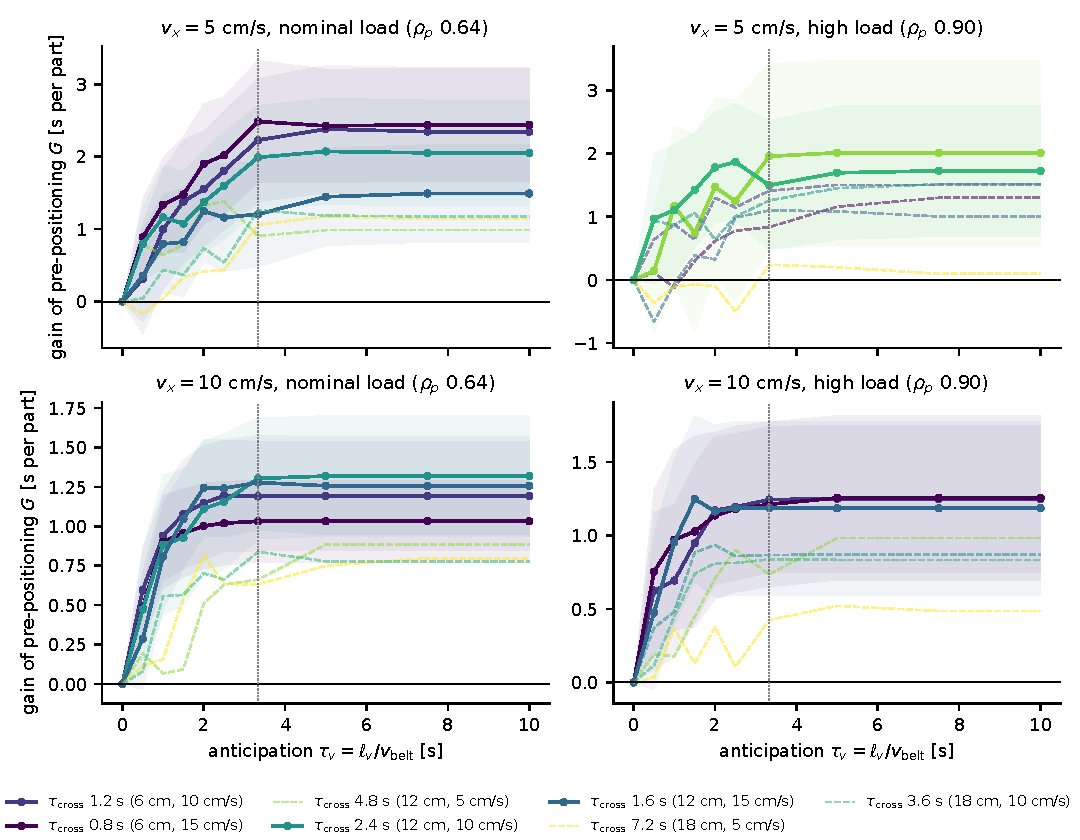
\includegraphics[width=\linewidth]{figures/bench_curves_poisson.pdf}
\caption{Geometry bench, \nj, Poisson arrivals: gain of pre-positioning $G$ [s per part]
against the anticipation, by crossing time (colour), for the two along-belt head speeds
(rows) and the two loads (columns). Solid lines with bands: cells worth sizing the coverage
for; dashed: undetermined. The dotted vertical line is 3.33~s, the anticipation of the
reference cell's whole entry zone.}
\label{fig:curves}
\end{figure}

\begin{figure}[t]
\centering
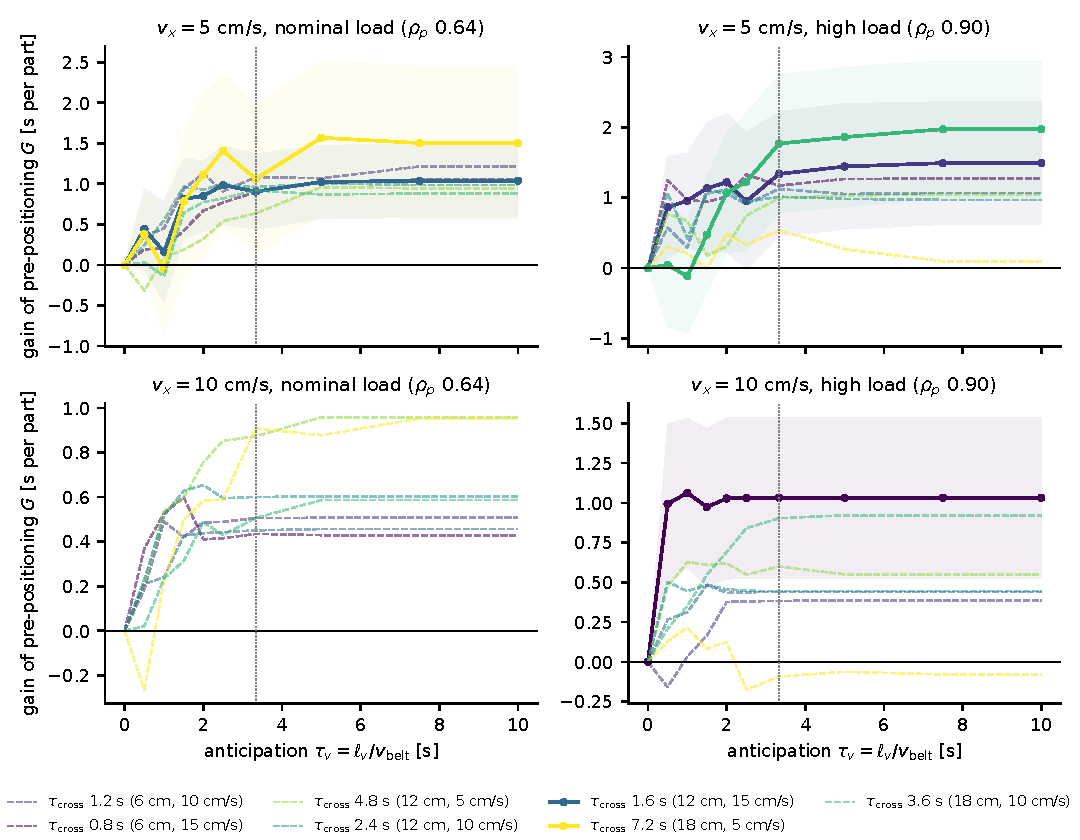
\includegraphics[width=\linewidth]{figures/bench_curves_burst.pdf}
\caption{Geometry bench, \nj, bursty arrivals: gain of pre-positioning $G(\tv)$ [s per part, 95\,\% band] against the anticipation, with the panels grouped by along-belt head speed and load and the units and markers of Figure~\ref{fig:curves} (Poisson arrivals).}
\label{fig:curvesburst}
\end{figure}

\begin{table}[t]
\centering\small
\caption{Geometry bench, \nj: sufficient coverage in the 18 cells worth sizing for.
Share at 3.33~s: $G(3.33\,\mathrm{s})/G(10\,\mathrm{s})$. Cost of 3.33~s:
$J_{\mathrm{when\_idle}}(\tau)-J_{\mathrm{when\_idle}}(10\,\mathrm{s})$, paired, bold when
its interval excludes zero. Knee: first grid anticipation retaining 90\,\% of
$G(10\,\mathrm{s})$, point estimate, and conservatively (lower simultaneous-95\,\% bound
$\ge0$; undet.\ = no grid point qualifies).}
\label{tab:sufficient}
\resizebox{\linewidth}{!}{% generated by experiments/paper2_bench_figures.py from data/geometry_bench.csv.gz
\begin{tabular}{@{}ccccl ccccc@{}}
\toprule
spacing & $v_y$ & $v_x$ & $\tau_{\mathrm{cross}}$ & load / arrivals & $G(10\,\mathrm{s})$ & share at 3.33~s & cost of 3.33~s & knee & knee (cons.) \\
{[cm]} & [cm/s] & [cm/s] & [s] & & [s/part] & [\%] & [s/part] & [s] & [s] \\
\midrule
6 & 10 & 5 & 1.2 & nominal / Poisson & $+2.35 \pm 0.88$ & 95 & $+0.12 \pm 0.18$ & 3.33 & 5.00 \\
6 & 10 & 5 & 1.2 & high / bursts & $+1.49 \pm 0.87$ & 90 & {\boldmath$+0.15 \pm 0.15$} & 5.00 & 7.50 \\
6 & 10 & 10 & 1.2 & nominal / Poisson & $+1.19 \pm 0.35$ & 100 & $+0.00 \pm 0.00$ & 1.50 & 2.50 \\
6 & 10 & 10 & 1.2 & high / Poisson & $+1.25 \pm 0.50$ & 100 & $+0.00 \pm 0.01$ & 2.00 & 3.33 \\
6 & 15 & 5 & 0.8 & nominal / Poisson & $+2.44 \pm 0.78$ & 102 & $-0.05 \pm 0.34$ & 3.33 & 5.00 \\
6 & 15 & 10 & 0.8 & nominal / Poisson & $+1.03 \pm 0.26$ & 100 & $+0.00 \pm 0.00$ & 1.50 & 2.00 \\
6 & 15 & 10 & 0.8 & high / Poisson & $+1.26 \pm 0.56$ & 96 & $+0.04 \pm 0.06$ & 2.00 & 5.00 \\
6 & 15 & 10 & 0.8 & high / bursts & $+1.03 \pm 0.51$ & 100 & {\boldmath$+0.00 \pm 0.00$} & 0.50 & 2.00 \\
12 & 5 & 5 & 4.8 & high / Poisson & $+2.02 \pm 1.47$ & 97 & $+0.06 \pm 0.27$ & 3.33 & undet. \\
12 & 10 & 5 & 2.4 & nominal / Poisson & $+2.05 \pm 0.73$ & 97 & $+0.06 \pm 0.12$ & 3.33 & 5.00 \\
12 & 10 & 10 & 2.4 & nominal / Poisson & $+1.32 \pm 0.38$ & 99 & $+0.01 \pm 0.02$ & 3.33 & 3.33 \\
12 & 15 & 5 & 1.6 & nominal / Poisson & $+1.49 \pm 0.67$ & 81 & {\boldmath$+0.29 \pm 0.23$} & 5.00 & 7.50 \\
12 & 15 & 5 & 1.6 & nominal / bursts & $+1.04 \pm 0.46$ & 87 & {\boldmath$+0.13 \pm 0.10$} & 2.50 & 5.00 \\
12 & 15 & 10 & 1.6 & nominal / Poisson & $+1.26 \pm 0.31$ & 102 & $-0.02 \pm 0.04$ & 2.00 & 2.00 \\
12 & 15 & 10 & 1.6 & high / Poisson & $+1.19 \pm 0.59$ & 100 & $+0.00 \pm 0.00$ & 1.50 & 2.50 \\
18 & 5 & 5 & 7.2 & nominal / bursts & $+1.50 \pm 0.95$ & 71 & {\boldmath$+0.44 \pm 0.33$} & 2.50 & 7.50 \\
18 & 10 & 5 & 3.6 & high / Poisson & $+1.73 \pm 1.04$ & 87 & $+0.23 \pm 0.47$ & 2.00 & 7.50 \\
18 & 10 & 5 & 3.6 & high / bursts & $+1.97 \pm 0.98$ & 90 & $+0.21 \pm 0.30$ & 5.00 & 7.50 \\
\bottomrule
\end{tabular}
}
\end{table}

\textbf{The conservative answer.} The knee that retains 90\,\% of the gain lies at
0.5--5~s as a point estimate (median 2.5~s over the 18 cells: 1.75~s at $v_x=10$ and 3.33~s at $v_x=5$~cm/s) and at 2.0--7.5~s conservatively (arrival-time tie-break, as everything in this section before Section~\ref{sec:tiebreak}), with
one cell undetermined ($d=12$, $v_y=5$, $v_x=5$, high load, Poisson, where no grid point
is conservatively at 90\,\%). The two answers differ because the curves are flat near
their top: a cell can retain 95\,\% of its gain at 3.33~s and still need 5--7.5~s before
the paired contrast against 90\,\% of the top is conservatively positive. The protocol fixed the conservative result as the headline: 17 of the 18 cells reached the 90\,\%
criterion with 2.0--7.5~s. The practical result below accompanies it.

\textbf{The practical answer.} In the 18 cells, giving the controller 3.33~s of
anticipation (10~cm of belt at 3~cm/s, the reference cell's entry zone) instead of 10~s
cost a median of 0.05~s per part and at most 0.44~s per part, the largest value observed
over the 18 cells (Table~\ref{tab:sufficient}; the cost is significant in 5 of the 18).
With 2.5~s the cost was a median 0.09 and at most 0.77~s per part (significant in 5); with
1.5~s a median 0.33 and at most 1.50 (significant in 10). In share terms, 3.33~s retained
71--102\,\% of the whole-grid gain (median 97\,\%), 2.5~s 62--108\,\% (median 94\,\%) and
5~s 94--104\,\% (a share above 100\,\% means that the shorter view scored better on these
realizations: sampling noise around a flat top, or a heuristic that does not respond
monotonically to the view). The two
readings belong together: the share says how much of the benefit a shorter view keeps,
the paired cost what the cell loses by it. Both ranges are those of the 18 cells evaluated
and are not a bound for cells outside the bench.

\subsection{Sensitivity to the tie-break and replication on fresh realizations}\label{sec:tiebreak}
The bench ran the rule with its legacy tie-break, the arrival time, which may precede
the first observation of a part (Section~\ref{sec:design}); the results above describe
that controller and were fixed before the run. After the run, as a retrospective
sensitivity analysis and not as a new confirmation, the rule was rerun on the same 60
realizations with the observable tie-break (the instant of first observation) and the
criteria of Section~\ref{sec:bench} unchanged: both modes at 10~s in all 56 distinct cells
(6\,720 episodes; the legacy rerun reproduces every archived cost within the $10^{-7}$~s per
part checked), then the eight shorter positive grid points in the 19 cells that passed the
benefit criterion under that key (18\,240 episodes); zero coverage was not rerun. Under the
observable key the pure-information contrast of the rule is no longer zero by
construction, since the tie-break depends on the coverage, so $G$ at each coverage is
measured against a baseline that can move with it.

The benefit criterion passes 19 cells instead of 18; 13 pass under both keys, 5 only
under the arrival-time key and 6 only under the observable one, so similar counts hide
eleven changes of membership. In the 19 cells (Table~\ref{tab:tiebreak}), 3.33~s instead
of 10~s cost a median of 0.04~s per part and at most 0.44~s (individual 95\,\% interval
$-0.01$ to 0.89; the maxima of the two keys come from different cells); no interval
excludes zero on the side of a loss, and one excludes it on the other side ($d/v_y/v_x=12/15/5$,
high load, bursts: the shorter view was cheaper by $0.54\pm0.39$~s per part). The share of
the gain retained at 3.33~s was 58--130\,\%. The conservative 90\,\% criterion is first met
before 10~s in 3 of the 19 cells (at 2, 7.5 and 7.5~s) and first at 10~s, the end of the
grid, in the other 16. Of the 13 cells that pass under both keys, all 13 certify before
10~s under the arrival-time key and 3 under the observable key. The change is not only one
of precision: the set of cells, the estimated curves and their uncertainty all change, and
in two cells ($18/10/5$ at the high load with bursts and at the nominal load with Poisson
arrivals) even the point estimate first reaches 90\,\% only at 10~s. A fixed heuristic need
not respond monotonically to a wider view, and under the observable key its baseline moves
with the coverage. A first certification at the last grid point describes the uncertainty
and the coverages tested in that cell; it does not show that 10~s of coverage is
physically required.

\textbf{Replication on fresh realizations.} The observable-key result was then replicated on
60 realizations not used before (seeds 43700--43759), with the seed range, the 56 cells, the
benefit screen, the grid, the paired contrasts and the interval rules fixed before the
run: both modes at 10~s in all 56 cells and the eight shorter positive grid points in the
cells that passed the screen (20\,160 episodes). Fourteen cells pass
(Table~\ref{tab:fresh}); 9 of them also passed with the observable key on the original
realizations, 10 with the arrival-time key, and 8 in all three analyses. Giving the
controller 3.33~s instead of 10~s cost a median of 0.09 and at most 0.47~s per part
($18/5/5$, nominal load, bursts; individual 95\,\% interval 0.02--0.91), with an interval
excluding zero in 2 of the 14 cells and an upper limit at or below 0.5~s per part in 9; the
share of the gain retained at 3.33~s was 67--117\,\%. The point estimate first reaches the
90\,\% criterion before 10~s in 13 of the 14 cells, the conservative criterion in 1
($6/15/10$, nominal load, Poisson arrivals, at 2~s); the other 13 first certify at 10~s. The
intervals are per cell, computed after the screen and without adjustment for choosing the
largest estimate, so the largest observed mean is not an upper limit for the family.

Table~\ref{tab:cohorts} sets the three analyses side by side. In all of them a view of
3.33~s cost little on average in the cells where pre-positioning pays, though not in every
cell; early certification of 90\,\% retention is a property of the arrival-time key; and
which cells pass the benefit screen is not stable across realizations. The cost of a
shorter view and the share of the gain it retains answer different design questions: the
first is what the cell loses, the second whether a fixed fraction of the benefit can be
guaranteed. The belt-speed bench (Section~\ref{sec:belt}) already used the observable key.

\begin{table}[t]
\centering\small
\caption{The three analyses of the 3~cm/s geometry bench with \nj: the prespecified run
(arrival-time tie-break), its retrospective rerun with the observable tie-break on the
same realizations, and the replication with the observable tie-break on fresh
realizations. Each analysis applies the benefit screen independently; knees and costs as
in Table~\ref{tab:sufficient}; the cost interval is the individual paired 95\,\% interval of
the cell with the largest estimated cost.}
\label{tab:cohorts}
\resizebox{\linewidth}{!}{%
\begin{tabular}{@{}lccccc@{}}
\toprule
analysis & pass the screen & knee $<10$~s & cons.\ knee $<10$~s & cost of 3.33~s, median & largest [95\,\% CI] \\
\midrule
arrival-time key, seeds 9000--9059 & 18/56 & 18/18 & 17/18 & 0.05 & 0.44 [0.11, 0.77] \\
observable key, seeds 9000--9059 & 19/56 & 17/19 & 3/19 & 0.04 & 0.44 [$-0.01$, 0.89] \\
observable key, seeds 43700--43759 & 14/56 & 13/14 & 1/14 & 0.09 & 0.47 [0.02, 0.91] \\
\bottomrule
\end{tabular}}
\end{table}

\begin{table}[t]
\centering\small
\caption{Geometry bench, \nj\ with the observable tie-break, retrospective rerun on the
same 60 realizations (seeds 9000--9059): the 19 cells that pass the benefit criterion under
that key. $G(10\,\mathrm{s})$ and the cost of 3.33~s ($J_{\mathrm{when\_idle}}(3.33\,\mathrm{s})-
J_{\mathrm{when\_idle}}(10\,\mathrm{s})$, positive when the shorter view costs more, with its
individual paired 95\,\% interval; bold when it excludes zero) in s/part; knees as in
Table~\ref{tab:sufficient}, with the 10~s end of the grid among the tested points.}
\label{tab:tiebreak}
\resizebox{\linewidth}{!}{% generated by experiments/closure_0_7_40/paper2_closure_tables.py from data/recheck_0_7_39_geometry.txt and data/closure_0_7_40/observable_short_cost_ci.txt
\begin{tabular}{@{}cccl cccc@{}}
\toprule
spacing & $v_y$ & $v_x$ & load / arrivals & $G(10\,\mathrm{s})$ & knee & knee (cons.) & cost of 3.33~s \\
{[cm]} & [cm/s] & [cm/s] & & [s/part] & [s] & [s] & [s/part] \\
\midrule
6 & 10 & 5 & high / Poisson & $+1.67$ & 5 & 10 & $+0.43 \pm 0.64$ \\
6 & 10 & 5 & nominal / Poisson & $+2.53$ & 3.33 & 10 & $+0.28 \pm 0.35$ \\
6 & 10 & 10 & high / Poisson & $+1.03$ & 1.5 & 10 & $-0.07 \pm 0.32$ \\
6 & 10 & 10 & nominal / Poisson & $+1.12$ & 1 & 2 & $-0.08 \pm 0.13$ \\
6 & 15 & 5 & high / Poisson & $+1.80$ & 2.5 & 10 & $+0.28 \pm 0.74$ \\
6 & 15 & 5 & nominal / Poisson & $+2.41$ & 3.33 & 10 & $-0.26 \pm 0.42$ \\
6 & 15 & 10 & high / Poisson & $+1.15$ & 1 & 10 & $+0.06 \pm 0.27$ \\
6 & 15 & 10 & nominal / Poisson & $+1.01$ & 1.5 & 7.5 & $-0.07 \pm 0.13$ \\
12 & 5 & 10 & nominal / Poisson & $+1.18$ & 2 & 10 & $+0.11 \pm 0.36$ \\
12 & 10 & 5 & nominal / Poisson & $+1.79$ & 5 & 10 & $-0.09 \pm 0.42$ \\
12 & 10 & 10 & nominal / Poisson & $+1.33$ & 2 & 7.5 & $+0.01 \pm 0.25$ \\
12 & 15 & 5 & high / bursts & $+1.45$ & 1.5 & 10 & {\boldmath$-0.54 \pm 0.39$} \\
12 & 15 & 5 & nominal / bursts & $+1.09$ & 1.5 & 10 & $+0.20 \pm 0.38$ \\
12 & 15 & 5 & nominal / Poisson & $+1.46$ & 7.5 & 10 & $+0.33 \pm 0.45$ \\
12 & 15 & 10 & high / Poisson & $+1.13$ & 1.5 & 10 & $-0.17 \pm 0.36$ \\
12 & 15 & 10 & nominal / Poisson & $+1.25$ & 1.5 & 10 & $-0.13 \pm 0.18$ \\
18 & 5 & 10 & nominal / bursts & $+1.10$ & 3.33 & 10 & $+0.07 \pm 0.23$ \\
18 & 10 & 5 & high / bursts & $+1.75$ & 10 & 10 & $+0.44 \pm 0.45$ \\
18 & 10 & 5 & nominal / Poisson & $+1.35$ & 10 & 10 & $+0.04 \pm 0.59$ \\
\bottomrule
\end{tabular}
}
\end{table}

\begin{table}[t]
\centering\small
\caption{Geometry bench, \nj\ with the observable tie-break, replication on 60 fresh
realizations (seeds 43700--43759): the 14 cells that pass the benefit criterion. Columns
as in Table~\ref{tab:tiebreak}.}
\label{tab:fresh}
\resizebox{\linewidth}{!}{% generated by experiments/closure_0_7_40/paper2_closure_tables.py from data/closure_0_7_40/paper2_prospective_cells.csv
\begin{tabular}{@{}cccl cccc@{}}
\toprule
spacing & $v_y$ & $v_x$ & load / arrivals & $G(10\,\mathrm{s})$ & knee & knee (cons.) & cost of 3.33~s \\
{[cm]} & [cm/s] & [cm/s] & & [s/part] & [s] & [s] & [s/part] \\
\midrule
6 & 10 & 5 & high / bursts & $+1.62$ & 2.5 & 10 & $+0.12 \pm 0.31$ \\
6 & 15 & 10 & high / Poisson & $+1.29$ & 1.5 & 10 & $+0.09 \pm 0.27$ \\
6 & 15 & 10 & nominal / Poisson & $+1.12$ & 1 & 2 & $+0.01 \pm 0.03$ \\
12 & 5 & 5 & nominal / bursts & $+1.36$ & 3.33 & 10 & $+0.05 \pm 0.45$ \\
12 & 10 & 5 & nominal / bursts & $+1.29$ & 3.33 & 10 & $-0.11 \pm 0.18$ \\
12 & 10 & 5 & nominal / Poisson & $+2.21$ & 7.5 & 10 & {\boldmath$+0.41 \pm 0.38$} \\
12 & 10 & 10 & nominal / Poisson & $+1.37$ & 7.5 & 10 & $+0.08 \pm 0.18$ \\
12 & 15 & 5 & nominal / bursts & $+1.34$ & 10 & 10 & $+0.26 \pm 0.42$ \\
12 & 15 & 5 & nominal / Poisson & $+1.57$ & 2.5 & 10 & $+0.10 \pm 0.25$ \\
12 & 15 & 10 & high / Poisson & $+1.63$ & 2 & 10 & $-0.19 \pm 0.33$ \\
12 & 15 & 10 & nominal / Poisson & $+1.21$ & 1.5 & 10 & $+0.06 \pm 0.09$ \\
18 & 5 & 5 & nominal / bursts & $+1.38$ & 7.5 & 10 & {\boldmath$+0.47 \pm 0.45$} \\
18 & 10 & 5 & nominal / Poisson & $+1.70$ & 5 & 10 & $+0.20 \pm 0.51$ \\
18 & 10 & 10 & nominal / Poisson & $+1.07$ & 2 & 10 & $-0.04 \pm 0.21$ \\
\bottomrule
\end{tabular}
}
\end{table}

\subsection{What predicts the required anticipation}\label{sec:predict}
Figure~\ref{fig:normalized} shows the 18 curves as shares of their whole-grid gain, once
against $\tv/\tcross$ and once against $\tv$ in seconds. Normalized by the crossing time
the curves fan out: fast heads saturate at 2--4 crossing times, slow heads well before
one. In seconds they lie in a narrower band. Figure~\ref{fig:knee} and
Table~\ref{tab:predictors} make the comparison quantitative on the point-estimate knees.

\begin{figure}[t]
\centering
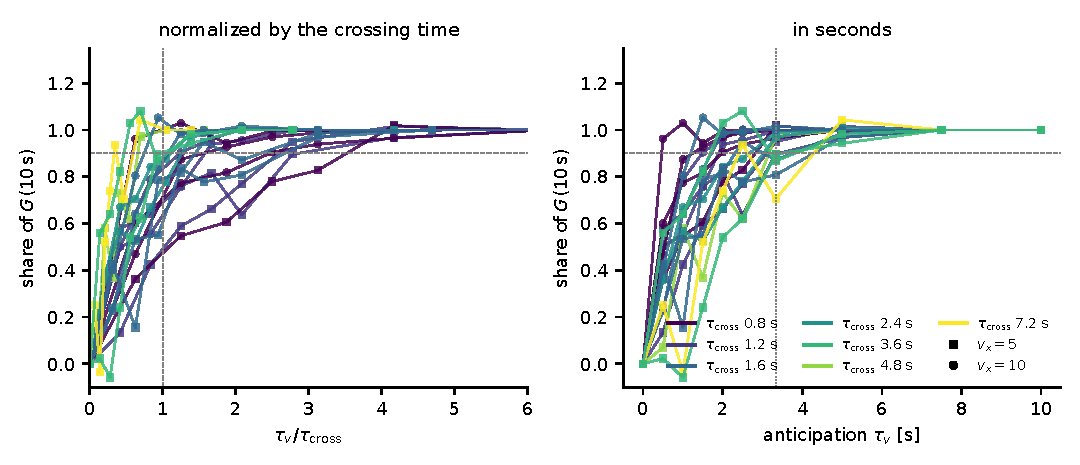
\includegraphics[width=\linewidth]{figures/bench_normalized.pdf}
\caption{Geometry bench, \nj, the 18 cells worth sizing for: share of the whole-grid gain
against the anticipation normalized by the crossing time (left) and in seconds (right).
Colour: $\tcross$; squares $v_x=5$, circles $v_x=10$~cm/s. The dashed horizontal line
is 90\,\%.}
\label{fig:normalized}
\end{figure}

\begin{figure}[t]
\centering
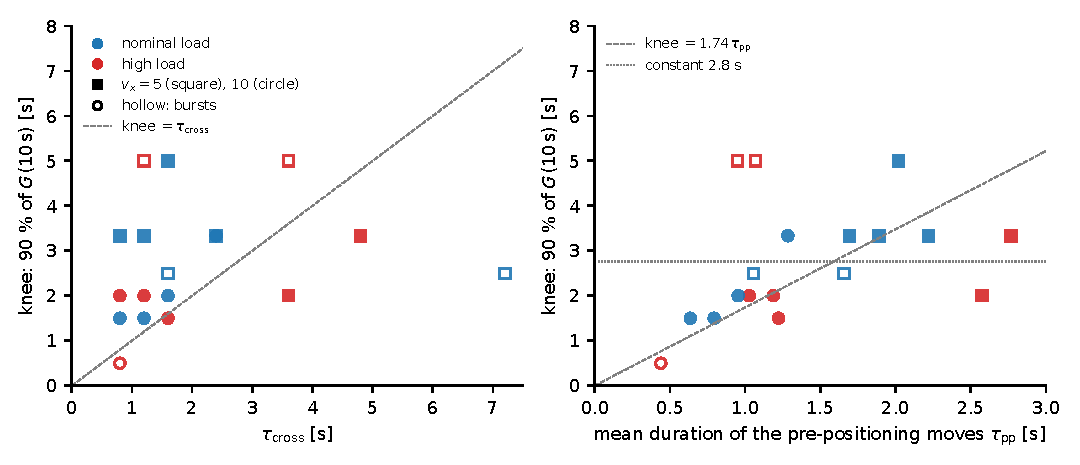
\includegraphics[width=\linewidth]{figures/bench_knee.pdf}
\caption{Geometry bench, \nj: the point-estimate knee (first grid anticipation
retaining 90\,\% of $G(10\,\mathrm{s})$) against the crossing time (left) and against the
mean duration of the pre-positioning moves actually made at 10~s of anticipation
(right), 18 cells. Lines: the identity, the fitted knee $=1.74\,\tpp$ and the constant.}
\label{fig:knee}
\end{figure}

\begin{table}[t]
\centering\small
\caption{Geometry bench, \nj: predictors of the knee over the 18 cells worth sizing for
(the 2.4~s triplet counted once). Leave-one-out mean absolute error of the knee predicted
from the other 17 cells; bold: lowest among the candidates fixed before the run. The last
row is a comparator computed after the run.}
\label{tab:predictors}
\resizebox{\linewidth}{!}{% generated by experiments/paper2_bench_figures.py from data/geometry_bench.csv.gz
\begin{tabular}{@{}lccc@{}}
\toprule
predictor & Spearman $\rho$ with the knee & leave-one-out MAE [s] & fitted coefficient \\
\midrule
knee $=\tau_{\mathrm{cross}}$ & $+0.38$ & 1.53 & --- \\
knee $=a\,\tau_{\mathrm{cross}}$ & $+0.38$ & 1.75 & $a=0.86$ \\
knee $=b\,\tau_{\mathrm{pp}}$ (mean planned duration of the moves started) & $+0.50$ & \textbf{1.02} & $b=1.74$ \\
knee $=b'\,(t_x+t_y)$ & $+0.47$ & 1.18 & $b'=1.33$ \\
knee $=$ constant & --- & 1.13 & $2.76$~s \\
knee $=$ mean of the other cells with the same $v_x$ (post hoc) & --- & 0.82 & --- \\
\bottomrule
\end{tabular}
}
\end{table}

By the frozen criterion the answer is the moves the head starts: $\tpp$ predicts the
knee with the lowest leave-one-out error (1.02~s), the crossing-time family with the
highest (1.53~s unscaled and 1.75~s rescaled, the poorest candidates, since the fitted
factor 0.86 is driven by the slow heads whose knees lie far below $\tcross$), and a
constant of 2.76~s in between (1.13~s), a serious comparator on these selected cells. A
comparator not fixed before the run does better than all of them: predicting each knee by
the mean knee of the other cells with the same along-belt head speed $v_x$, a quantity known
at design time, gives a leave-one-out error of 0.82~s (group means 3.53~s at $v_x=5$ and
1.79~s at $v_x=10$~cm/s; computed after the run from the knees of
Table~\ref{tab:sufficient}, on the same selected cells, with two observed speeds). The
trace-based predictor is therefore the best of the prespecified candidates, not the best
available description, and any general claim about a predictor needs held-out geometries.
The ranking also depends on the controller version and the cohort: on the 19 cells of the
observable key (Section~\ref{sec:tiebreak}; point-estimate knees, factor refitted in
every fold), the move duration gives 1.72~s, the group mean by $v_x$ 1.74~s, the crossing
time 2.12~s and the constant 2.27~s. Since the rerun changes both the policy and the
selected cells, this comparison does not isolate why the ranking changes. All these
errors concern the point-estimate knee; the conservative knee was not used as a target.
The rank correlations point the same way and are all moderate: 0.38 for $\tcross$, 0.50
for $\tpp$ and 0.47 for $t_x+t_y$, the supplementary sum of the two axis times (average
ranks for ties, since the knee takes values on the grid).\footnote{Draft 0.6 of this paper reported $+0.47$, $+0.53$ and $+0.51$, computed
with ties broken by position; the values here use average ranks. The leave-one-out errors
are unchanged.} The fitted factor, knee $\approx1.74\,\tpp$, is an empirical adjustment on
these 18 traces and not a mechanism: $\tpp$ is the planned duration recorded when a move
is decided, averaged per episode and then over the episodes with at least one move, so
that each such episode weighs equally (weighting each move equally instead gives a
factor of 2.00 and a leave-one-out error of 1.06~s, a sensitivity computed after the
run); the knee it predicts is the point-estimate grid point, not the conservative
coverage of Table~\ref{tab:sufficient}; and it needs full-view traces, which a designer
without a simulation of the cell does not have. The two errors belong together: 1.02~s
for the move duration, 1.13~s for the constant. Two qualifications the data impose. No predictor
is precise: the errors are two to three steps of the fine end of the grid (0.5~s steps up to 2.5~s; the grid is not uniform beyond), and the knee$/\tpp$
ratios range from 0.8 to 2.6 with two cells at 4.7--5.3. And $\tpp$ beats the constant by
0.1~s only, a small advantage: for a designer without traces, ``about 3~s of anticipation
at these loads'' is nearly as good as ``about 1.7 times the mean move''. The crossing time is the worst candidate because it ignores
the along-belt component of the moves, which the next section shows to be of the same
order as the lane change; the moves are $y$-dominated in 7--57\,\% of the cases (each
episode with moves weighted equally; weighting each move equally gives about
6--53\,\%, computed after the run), never a majority at $v_x=5$~cm/s.

\textbf{Same crossing time, same coverage?} Yes, and trivially so for the rule: check (iv)
of Section~\ref{sec:design} shows that cells with the same $\tcross$ and the same $x$
geometry are identical realization by realization, because with simultaneous axes the
geometry enters the dynamics only through the lane travel times. The question is
answered by the model's structure, not by the data; the informative comparison is across
different crossing times and along-belt speeds, which is what the rest of the bench does.

\subsection{The along-belt axis is a first-order factor}\label{sec:vx}
At the nominal load with Poisson arrivals, halving $v_x$ from 10 to 5~cm/s multiplied
the gain of pre-positioning by 1.2--2.4 in the four geometries ($\tcross\le2.4$~s) in
which both speeds pass the benefit criterion (1.03--1.32 $\to$ 1.49--2.44~s per part; by
1.1--1.5 in the three geometries in which neither does), lengthened the mean along-belt
component of the moves from 0.44--0.76 to 1.57--1.90~s in those four cells, lowered the
head's idle fraction under \texttt{none} from 17--27\,\% to 12--15\,\% (under
\texttt{when\_idle}, from 5--6 to 4--5\,\%), and moved the knee (arrival-time tie-break) from 1.5--3.33~s
(conservatively 2.0--3.33) to 3.33--5~s (conservatively 5--7.5). The size of the change
depends on the geometry; its direction does not.
The reference study had found that a head twice as slow on \emph{both} axes needed the
whole entry zone; the bench's pilot, which slowed the transverse axis alone, had found no
such need. The two are reconciled by the $x$ axis: the anticipation the camera must give
is set by the whole move, and the along-belt part of it does not scale with the belt
spacing.

\subsection{Mechanism}\label{sec:mechanism}
The traces show why the curves have the shape they have. The \emph{number} of
pre-positioning moves hardly depends on the anticipation (in the pilot, 24.6 moves per
episode at 0.2~s of anticipation and 27.7 at 3.3~s for the fastest head; 2.7 and 4.0 for
the slowest): almost every idle period of the head finds a visible part even with a tiny
window, so the opportunities are fixed by the head's idle time (under \texttt{none}, 5--33\,\% of
the time across the 56 cells, falling with the load and with slower heads), not by the
camera. What grows with
the anticipation, and saturates, is the gain per opportunity. That gain, an aggregate
ratio (seconds saved summed over all parts, divided by the number of moves), exceeds the
move's own duration several times over. With the number of unfinished parts recorded at
each move, the implied saving per part (aggregate gain per move divided by the parts in
the system at the move) is 1.0--2.0 times the move's duration in all ten cells worth sizing
for at the nominal load: the aggregate ratio is compatible with the saving of a move being
transmitted to the parts queued behind it, which is what the check frozen before the run asked
for; it does not show the transmission itself, which would need the delay of each queued
part to be traced. At the high load the ratio is 3.5--9.5 in the five Poisson cells (2.5--6.8 moves per
episode, head idle 6--10\,\% under \texttt{none}, aggregate gain per move 20--87~s) and
2.1--2.5 in the three bursty cells (13--17 moves per episode, idle 14--20\,\%, 7--17~s per
move): there the aggregate gain per move is more than the queue at the move explains, the transmission reading is not supported, and we keep the measured
effect without an interpretation. That one early service at high load prevents a cascade
of belt stops which delays parts arriving later than the count at the move sees is a
hypothesis, not tested here.

\subsection{Physical entry length}\label{sec:entry}
The bench's 35~cm entry zone is 25~cm longer than the reference cell's. On the reference
geometry, with the same visible lengths and the same arrivals at the feed point, the
longer entry adds $+10.35\pm0.52$ (nominal, Poisson), $+11.11\pm0.55$ (nominal, bursts),
$+13.19\pm0.71$ (high, Poisson) and $+11.69\pm0.64$~s per part (high, bursts) to the
rule's penalized flow time $J$ (Table~\ref{tab:entry}; on the raw flow time $+10.60\pm0.40$,
$+11.15\pm0.50$, $+13.34\pm0.67$ and $+11.74\pm0.65$): 8.33~s of it is the free transit at
3~cm/s, and the remaining 2.0--4.9~s, which grow with the load, are not decomposed by
the data: they contain the belt stops acting on the parts of the longer entry zone, any
change of dispatch, and the change of the penalty term. No difference in the gain of pre-positioning at a given anticipation was detected
between the two entry lengths: the paired differences are at most $\pm0.23$~s per part
(nominal) and $\pm0.46$ (high), with intervals that include zero at every grid point
(Table~\ref{tab:entry}). We read this, within the precision of those intervals, as the
bench measuring the camera's reach rather than the installation; where a percentage is given it uses as denominator the configuration's own \texttt{none} level minus its free transit $\ell_{\mathrm{entry}}/\vb$ (10/3~s for the 10~cm entry, 35/3~s for the 35~cm entry at 3~cm/s); the 25/3 = 8.33~s above is the paired change of the transit, not a denominator.

\begin{table}[t]
\centering\small
\caption{Physical-length check, \nj, reference geometry ($d=12$~cm, $v_x=v_y=10$~cm/s):
the 35~cm entry against the 10~cm entry, same visible lengths, same arrivals at the feed
point. $\Delta$ `none' level: penalized flow time $J$ added by the longer entry; $\Delta G$: difference
of the pre-positioning gain at the same anticipation (35~cm minus 10~cm), paired, 95\,\%
CI.}
\label{tab:entry}
\resizebox{\linewidth}{!}{% generated by experiments/paper2_bench_figures.py from data/geometry_bench.csv.gz
\begin{tabular}{@{}llcccc@{}}
\toprule
load & arrivals & $\Delta$ `none' level (35 $-$ 10~cm) & $\Delta G$ at 1~s & $\Delta G$ at 2~s & $\Delta G$ at 3.33~s \\
 & & [s/part] & [s/part] & [s/part] & [s/part] \\
\midrule
nominal & Poisson & $+10.35 \pm 0.52$ & $-0.08 \pm 0.48$ & $-0.14 \pm 0.53$ & $-0.04 \pm 0.52$ \\
nominal & bursts & $+11.11 \pm 0.55$ & $-0.10 \pm 0.37$ & $-0.14 \pm 0.39$ & $-0.23 \pm 0.39$ \\
high & Poisson & $+13.19 \pm 0.71$ & $-0.14 \pm 0.77$ & $+0.46 \pm 0.81$ & $+0.38 \pm 0.78$ \\
high & bursts & $+11.69 \pm 0.64$ & $-0.26 \pm 0.49$ & $-0.19 \pm 0.56$ & $-0.26 \pm 0.57$ \\
\bottomrule
\end{tabular}
}
\end{table}

\subsection{The network as a secondary controller}\label{sec:benchnet}
The network's curves rise and saturate like the rule's, with gains of the same order
($G(10\,\mathrm{s})$ 0.13--1.68~s per part over the 72 regimes, 0.38--1.68 at the nominal
load), but they are noisier and saturate more slowly: it passes the benefit criterion in
17 of the 72 regimes (14 at the nominal load, 14 with Poisson, 13 with $v_x=5$; $G$
1.01--1.68 in those), its point-estimate knees lie at 1--10~s, and its conservative knee is never
reached before 10~s. No predictor works for it (Spearman correlations $\le0.14$). The
value of widening the view with the network's mode input fixed,
$J_{\mathrm{when\_idle}}(0)-J_{\mathrm{when\_idle}}(\tv)$, is of the same size as $G$ at the
nominal load (e.g.\ $+1.03\pm0.49$ against $G=+1.13\pm0.58$ at $d=6$, $v_y=5$, $v_x=5$;
two estimates of different quantities, whose paired difference was not computed, and a
fixed-mode contrast and a mode-change contrast answer different questions). The value of seeing with
the same actions, $J_{\mathrm{none}}(0)-J_{\mathrm{none}}(\tv)$, lies between $-0.37$ and
$+0.71$~s per part at the nominal load (7 of the 36 cell--arrival combinations outside
$\pm0.3$) and is positive at the high load with bursts (up to $+1.6$~s per
part, significant in 5 of 9 cells at each $v_x$; Table~\ref{tab:net}), consistent with
the one significant B-vs-A cell of the reference study (heavy load, bursts). In the levels, with
\texttt{when\_idle} at 10~s the network's penalized flow time lies below the rule's in 71
of the 72 regimes (significantly in 70), by 3.1--11.1~s per part at $v_x=5$~cm/s and by
0.2--4.9 at $v_x=10$, and above it in one ($d=18$, $v_y=5$, $v_x=10$, high load, Poisson,
$+1.3\pm1.1$); this comparison with the rule does not by itself quantify any degradation
of the network outside its training ranges.

\begin{table}[t]
\centering\small
\caption{Geometry bench, network: per block of $v_x\times$load$\times$arrivals (nine
geometries each), the number of cells worth sizing for, the range of $G(10\,\mathrm{s})$,
the range of the point-estimate knee in those cells, and the range of the value of seeing
with the same actions, $J_{\mathrm{none}}(0)-J_{\mathrm{none}}(10\,\mathrm{s})$ [s per
part], with the number of cells in which it is significantly positive (cells in which it
is significantly negative, one in each of four blocks, are not counted).}
\label{tab:net}
\resizebox{\linewidth}{!}{% generated by experiments/paper2_bench_figures.py from data/geometry_bench.csv.gz
\begin{tabular}{@{}lllcccc@{}}
\toprule
$v_x$ & load & arrivals & useful cells & $G(10\,\mathrm{s})$ range & knee range & seeing, `none'(0) $-$ `none'(10~s) \\
{[cm/s]} & & & (of 9) & [s/part] & [s] & [s/part], range \\
\midrule
5 & nominal & Poisson & 8 & +0.56 to +1.68 & 1.0--7.5 & -0.37 to +0.71 (1 sig.) \\
5 & nominal & bursts & 2 & +0.38 to +1.45 & 3.3--10.0 & -0.10 to +0.58 (1 sig.) \\
5 & high & Poisson & 3 & +0.39 to +1.58 & 2.0--7.5 & -0.38 to +1.11 (1 sig.) \\
5 & high & bursts & 0 & +0.13 to +0.93 & --- & +0.01 to +1.58 (5 sig.) \\
\midrule
10 & nominal & Poisson & 3 & +0.67 to +1.13 & 1.0--2.0 & -0.25 to +0.36 (0 sig.) \\
10 & nominal & bursts & 1 & +0.42 to +1.10 & 7.5--7.5 & -0.22 to +0.25 (1 sig.) \\
10 & high & Poisson & 0 & +0.26 to +1.68 & --- & -1.18 to +0.78 (4 sig.) \\
10 & high & bursts & 0 & +0.19 to +0.63 & --- & -0.51 to +0.89 (5 sig.) \\
\bottomrule
\end{tabular}
}
\end{table}

\subsection{Belt speed: what transfers to 5~cm/s}\label{sec:belt}
Table~\ref{tab:belt} and Figure~\ref{fig:belt} give the belt-speed bench of
Section~\ref{sec:beltdesign} (11\,520 episodes; no candidate upstream of the visible
stretch, identical arrivals at both speeds in all 240 cell--realization pairs,
\texttt{when\_idle} equal to \texttt{none} at zero length exactly). Its check column
reproduces the 3~cm/s costs of Section~\ref{sec:howmuch} with the 50~cm entry: $C_3(10\,
\mathrm{cm})$ is $+0.10\pm0.47$, $+0.18\pm0.23$, $-0.15\pm0.26$ and $-0.11\pm0.17$~s per
part in the four cells, every interval containing the value of the geometry bench. At
5~cm/s, \textbf{10~cm of coverage cost less than the margin in the two cells with
$v_x=10$~cm/s}: the upper 95\,\% bounds of $C_5(10\,\mathrm{cm})$ are 0.33 and 0.23~s per
part, below the margin of 0.5 ($H_{\mathrm{cm}}$, conservative), and no difference
between 16.7 and 10~cm was detected there (direct paired contrast 10 minus 16.7~cm:
$+0.09\pm0.26$ and $+0.05\pm0.14$~s per part). The 90\,\% retention criterion, however,
is not certified at 10~cm in either fast cell at 5~cm/s: the first conservatively
certified length is 25~cm in $d=12$, $v_y=10$, $v_x=10$ and 50~cm in $d=6$, $v_y=15$,
$v_x=10$; the margin and the certification are different questions
(Section~\ref{sec:beltdesign}). As written beforehand, these two cells cannot separate the two scales,
so their result is the practical one, 10~cm suffice at 5~cm/s, not a mechanistic one.
\textbf{At 5~cm/s, neither of the two slow-axis cells met the benefit criterion with
the full view; the paired comparison between speeds detected a reduction in one of the
two.} $G_5(50\,\mathrm{cm})=+0.62\pm0.73$ and $+0.47\pm0.55$~s per part, against
$+1.74\pm0.87$ and $+1.58\pm0.89$ at 3~cm/s; paired across speeds, 3 minus 5~cm/s, the
difference is $+1.12\pm1.21$ in $d=12$, $v_y=10$, $v_x=5$ (not detected) and
$+1.11\pm1.02$ in $d=6$, $v_y=15$, $v_x=5$ (detected). The frozen verdict, named ``benefit lost at this speed'' in the protocol and reported
in Table~\ref{tab:belt} as ``full-view benefit criterion not met at 5~cm/s'', follows
from the precedence of the benefit criterion, so the coverage question
is moot there; on the shorter views themselves the conservative reading is undetermined,
not ``within the margin'': $C_5(16.7\,\mathrm{cm})=+0.12\pm0.39$ and $+0.12\pm0.45$~s per
part have upper bounds of 0.51 and 0.57, above the margin, with point estimates inside
it, so $H_{\mathrm{neither}}$ is neither established nor excluded. In the other two
cells the full-view benefit rose at the faster belt in $d=12$, $v_y=10$, $v_x=10$
($-0.77\pm0.60$) and no difference was detected in $d=6$, $v_y=15$, $v_x=10$
($-0.06\pm0.53$).
\textbf{The comparison between centimetres and seconds remains open}: the cells that
could have separated the two readings are the ones that lost the benefit, and the
descriptive alignment reading fixed beforehand (mean absolute difference of the shares
of the full-view gain retained at matched lengths and at matched anticipations) favours
the time scale in three cells and the distance scale in one, with a post hoc caveat
recorded in the methods documentation that the matched-anticipation pairs sit where both
curves are flatter. One premise check: with the 50~cm entry, the cell $d=12$, $v_y=10$, $v_x=10$ sits
on the benefit threshold at 3~cm/s ($+0.99\pm0.38$ against the criterion's 1.0, lower
bound 0.61 against 0.5) and is reported as it falls. The traces are compatible with the
interception moving downstream at the faster belt (the planned along-belt component of
the pre-positioning moves grows from 1.5--1.8 to 2.3--2.5~s in the $v_x=5$ cells and from
0.5--0.7 to 0.8--1.0~s in the $v_x=10$ cells, the transverse component is unchanged, the
head's idle share and the number of moves fall); this is a reading of the traces, not a
tested hypothesis. One more difference from the geometry bench, found by a referee:
this bench ran with the observable tie-break of the rule (Section~\ref{sec:design}), so
the rule's \texttt{none} level itself depends on the visible length here, which it did
not in the geometry bench (identical across lengths by construction). The mean changes
$J_{\mathrm{none}}(0)-J_{\mathrm{none}}(50\,\mathrm{cm})$ lie within $\pm0.41$~s per part
over the eight cell--speed pairs and are detected in one ($-0.21\pm0.17$ at $d=6$,
$v_y=15$, $v_x=10$, 5~cm/s); $G_v(\ell)$ is defined at each length against its own
\texttt{none} level and is unaffected as a definition, but ``seeing without acting'' is
no longer zero by construction in this study, and the geometry and belt-speed benches
differ in seed range, entry length and rule version.

\begin{table}[t]
\centering\small
\caption{Belt-speed bench, \nj, nominal load, Poisson arrivals, 50~cm entry, 60 paired
realizations (seeds used once): the full-view benefit $G_v(50\,\mathrm{cm})$ at 3 and at
5~cm/s with the benefit criterion, the paired costs at 5~cm/s of 10~cm (2.00~s) and
16.7~cm (3.33~s) against 50~cm, the check column $C_3(10\,\mathrm{cm})$ (the 3.33~s cost at
3~cm/s, to be compared with Section~\ref{sec:howmuch}), and the frozen verdict
(conservative reading, margin 0.5~s per part). Seconds per part, 95\,\% CI.}
\label{tab:belt}
\resizebox{\linewidth}{!}{% generated by experiments/paper2_bench_figures.py from data/belt_speed_bench.csv.gz
\begin{tabular}{@{}lcccccccl@{}}
\toprule
cell & $G_3(50\,\mathrm{cm})$ & useful at 3 & $G_5(50\,\mathrm{cm})$ & useful at 5 & $C_5(10\,\mathrm{cm})$ & $C_5(16.7\,\mathrm{cm})$ & $C_3(10\,\mathrm{cm})$ & verdict at 5~cm/s \\
 & [s/part] & & [s/part] & & $=2.00$~s & $=3.33$~s & $=3.33$~s (check) & (conservative) \\
\midrule
$d=12$, $v_y=10$, $v_x=5$ ($\tcross=2.4$~s) & $+1.74 \pm 0.87$ & yes & $+0.62 \pm 0.73$ & no & $-0.00 \pm 0.51$ & $+0.12 \pm 0.39$ & $+0.10 \pm 0.47$ & full-view benefit criterion not met at 5~cm/s \\
$d=12$, $v_y=10$, $v_x=10$ ($\tcross=2.4$~s) & $+0.99 \pm 0.38$ & no & $+1.76 \pm 0.39$ & yes & $+0.06 \pm 0.26$ & $-0.02 \pm 0.24$ & $+0.18 \pm 0.23$ & 10~cm keep the benefit ($H_{\mathrm{cm}}$) \\
$d=6$, $v_y=15$, $v_x=5$ ($\tcross=0.8$~s) & $+1.58 \pm 0.89$ & yes & $+0.47 \pm 0.55$ & no & $+0.48 \pm 0.55$ & $+0.12 \pm 0.45$ & $-0.15 \pm 0.26$ & full-view benefit criterion not met at 5~cm/s \\
$d=6$, $v_y=15$, $v_x=10$ ($\tcross=0.8$~s) & $+1.16 \pm 0.34$ & yes & $+1.22 \pm 0.37$ & yes & $+0.05 \pm 0.18$ & $+0.00 \pm 0.14$ & $-0.11 \pm 0.17$ & 10~cm keep the benefit ($H_{\mathrm{cm}}$) \\
\bottomrule
\end{tabular}
}
\end{table}

\begin{figure}[t]
\centering
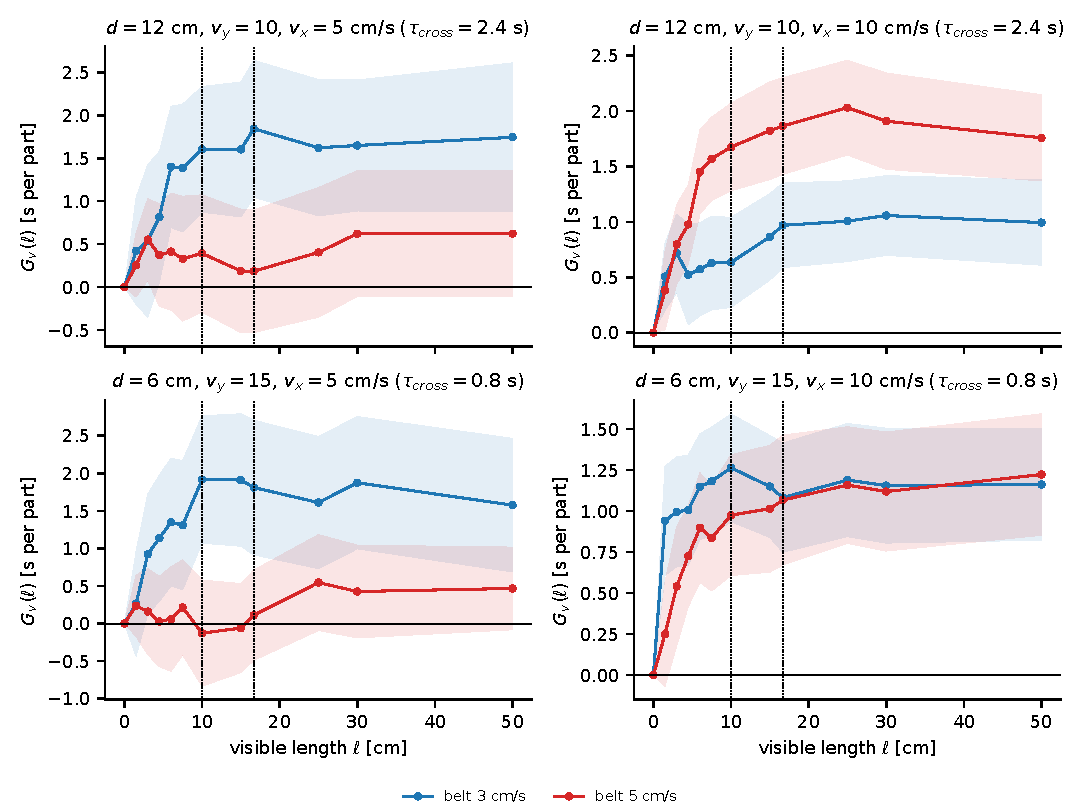
\includegraphics[width=\linewidth]{figures/bench_belt.pdf}
\caption{Belt-speed bench, \nj: the gain of pre-positioning $G_v(\ell)$ [s per part, 95\,\%
band] against the visible length in centimetres, belts at 3 and 5~cm/s, the same arrival
realizations at both speeds, four cells. Dotted lines at 10 and 16.7~cm; the same
10~cm are 3.33~s of anticipation at 3~cm/s and 2.00~s at 5~cm/s.}
\label{fig:belt}
\end{figure}

%====================================================================
\section{Discussion}\label{sec:discussion}
%====================================================================

The discussion turns the results into a specification in seconds, explains why widening the view alone changed little, reads the effect of load, bursts and idle time, and states the limits.

\subsection{A specification in seconds}
The results give the numbers for a specification of the camera's reach in seconds of
anticipation. In the 18 cells that pass the benefit criterion, 3.33~s of anticipation cost
a median 0.05 and at most 0.44~s per part against a view three times longer (the largest
value observed), and retained 71--102\,\% of the estimated gain; the conservative
requirement to retain 90\,\% of the gain (Table~\ref{tab:sufficient}) is 2--5~s in the
cells with $v_x=10$~cm/s and 5--7.5~s in those with $v_x=5$~cm/s, plus one cell with
$v_x=5$ unresolved within the grid. Those numbers belong to the rule with the
arrival-time tie-break. For a camera-based controller, the retrospective rerun with the
observable key (Section~\ref{sec:tiebreak}) supports the first statement (a median of
0.04 and at most 0.44~s per part for 3.33~s) but not the second: only 3 of its 19 cells
certify 90\,\% before 10~s; the replication on fresh realizations agrees (a median of 0.09
and at most 0.47~s per part; 1 of 14 cells certifies before 10~s). Every cell of the geometry bench runs its belts at 3~cm/s, so
within it seconds of belt motion and centimetres are one unit ($\lv=3\tv$); the clock time a
camera gives is longer whenever the belt stops (Section~\ref{sec:anticipation}). The physical argument
for seconds is that the quantity the anticipation must cover is the head's move, which
does not depend on $\vb$; but changing $\vb$ also changes where the head intercepts each
part, and the curve may move with it. The belt-speed bench (Section~\ref{sec:belt}) gives
the practical answer for 5~cm/s without settling the scale: 10~cm cost less than the
margin of 0.5~s per part against the full view in the two cells with the fast along-belt
axis (whose conservative requirement at 3~cm/s in the geometry bench, nominal load and
Poisson arrivals, is 2.0 and 3.33~s with the arrival-time key, 7.5~s with the observable
key on the same realizations, and 2 and 10~s with that key on fresh realizations; in the
belt-speed bench, with its 50~cm entry, the cell $12/10/10$ misses the benefit
criterion at 3~cm/s, $+0.99$~s per part), while the conservative
90\,\% criterion was not certified at 10~cm in either of them (first certified at 25 and
50~cm); in the two cells with the
slow axis the full-view benefit itself fell below the criterion at 5~cm/s, a reduction
detected in one of them. Whether 2~s or
10~cm is the right reading of ``10~cm'' therefore remains open, and the specification
below is stated at 3~cm/s with that practical extension to 5~cm/s. The pilot's reference, the transverse
crossing time, is rejected as a predictor: it misses the along-belt part of every move,
and it would mis-size the coverage by 1.5~s on average over the cells tested, three grid
steps. Among the predictors fixed before the run, the planned duration of the moves the
head starts, both axes included, predicts the point-estimate requirement best on the 18
cells of the arrival-time key (fitted factor 1.7 on its mean), but only 0.1~s better than
a constant, and a post hoc group mean by along-belt head speed does better (0.82~s); on the
19 cells of the observable key (seeds 9000--9059) the move duration and that group mean are within 0.03~s
(1.72 and 1.74~s). The data therefore support a number of seconds for the family of cells
tested, not a predictor to extrapolate to cells that differ much from those tested.

\subsection{Why widening the view alone changes little}
Under treatment~B the controller must choose among the parts already in the zone
whenever there is one; upstream visibility can help it only through the order of the
zone parts. For the rule with the arrival-time tie-break this help is zero by construction;
an average near zero for the network measures what this policy extracts from the view, not
what an optimal policy could. Treatment A to B changes the view with the same permission
to act, B to C adds the permission to act for a fixed view, and D bounds what more
information could give a policy able to use it; a fixed policy's measured score need not
be optimal. In the reference cell that is worth little (Section~\ref{sec:seeing}); in the
bench the rule with the arrival-time key cannot use it at all (with the observable key the
view can change its tie-breaks), and the network's value of seeing with the same
actions lies within $\pm0.7$~s per part at the nominal load (7 of 36 cell--arrival
combinations outside $\pm0.3$). The exception is the high load
with bursts, where the network gains up to 1.6~s per part from the view alone: when the
belts queue and the parts arrive in groups, knowing what is about to enter lets the
controller finish near the belt that will need it. That is the regime in which the
reference study also found its one significant B-vs-A cell.

\subsection{Load, bursts and idle time}
Pre-positioning is an action for an idle head. The number of opportunities is fixed by
the head's idle time, which falls with the load and with slower heads, and bursts spend
the opportunities on the first part of each burst. This is why the cells worth sizing for
are concentrated at Poisson arrivals, why the high-load cells are mostly undetermined by
precision, and why the gain per opportunity grows with the load: a second saved on the
head's cycle can be saved by every part queued behind it. The traces are compatible with
that reading at the nominal load; at the high load the queue count does not account for
the size of the effect, and the mechanism there is open.

\subsection{Limits}\label{sec:limits}
The results are for one family of cells (three belts, a 35~cm laser zone, constant
processing of 2.5~s) and two loads. The geometry bench used a belt at 3~cm/s; the
reference study used 3~cm/s at the nominal load and 5~cm/s at the heavy load; the third
study compared both speeds at the nominal load. The specification in seconds has been
tested within the grid of Section~\ref{sec:bench} and not beyond it, so the
recommendation is for cells of this family at 3~cm/s, with the belt-speed bench of
Section~\ref{sec:belt} as its only test at 5~cm/s: four cells, the nominal load, Poisson
arrivals and the rule alone, in which 10~cm cost less than the margin where the
full-view benefit passed the criterion, and which left the choice between centimetres and seconds open,
because the cells that could separate the two scales lost the benefit at 5~cm/s. A bench
that keeps a useful benefit at both speeds in cells with a slow along-belt axis (a lower
load, or a longer laser zone) would be the experiment that settles the scale. Thirty-eight of the
56 cells are left undetermined, some because the gain is small (bursts at the nominal
load) and some because 60 realizations do not resolve it (the high load); a study of the
high load alone would need more realizations and a new reserved range. The penalty
weights are placeholders in equivalent seconds; since the gain is almost entirely flow
time, the coverage costs and knees are reported on $J$ as frozen; the benefit screen is
not insensitive to the weights: scored on the raw flow time instead of $J$, 15 cells pass
it instead of 18 (a sensitivity computed after the run). An economic translation (the break-even
cost of the camera's reach against the seconds saved per part at the cell's throughput)
needs the cell's operating costs and is deferred. The study measures the \emph{reach} of
the camera, not its precision: detection noise, latency and losses are a separate
question. The designs are a predefined grid compared on paired realizations, not optimized
jointly with the controller as line parameters are in \cite{Sarker2001}. The reading of the
gain per move as a saving passed on to the parts queued behind it is a compatibility
argument; demonstrating it would need paired alternative moves from matched states. Parts
are points with a minimum spacing, the head has no acceleration, and the learned policy is a
secondary controller whose training ranges the bench partly exceeds.
The rule's tie-break differs between studies, the arrival time in the first two and the
observable instant in the third (Sections~\ref{sec:design} and \ref{sec:belt}); the
retrospective rerun of the geometry bench with the observable key
(Section~\ref{sec:tiebreak}) shows that its certified coverage depends on that choice, and
the replication on fresh realizations that the set of cells passing the benefit criterion
changes with the realizations. The three sets of reserved realizations were used once for
their prespecified analyses; those of the geometry bench were reused for the retrospective
rerun, and the replication used a fourth, fresh set.

%====================================================================
\section{Conclusions}
%====================================================================
For a shared-head cell over parallel conveyors, the value of a camera that sees upstream
of the working zone is mostly the value of the action it enables, not of the information
it adds: in the reference cell, widening the view without the action produced small
effects, while allowing the idle head to move towards a visible part reduced the
penalized flow time by 7.4\,\% at the nominal load for both a dispatching rule and a
learned policy (2.8--4.3\,\% for the network and 2.7--3.9\,\% for the rule with bursts
or a slow head). Across 56 distinct cells with belt
spacings of 6--18~cm, transverse head speeds of 5--15~cm/s, along-belt speeds of 5 and
10~cm/s, two loads and two arrival processes, pre-positioning passes the benefit criterion
in 18, 13 of them with Poisson arrivals; in those, 3.33~s of anticipation cost a median
0.05 and at most 0.44~s per part against 10~s (the largest value observed). Seventeen of
the 18 configurations reached the conservative criterion of retaining 90\,\% of the
gain, with coverages of 2 to 7.5~s, the slow along-belt axis needing the most; one is
unresolved within the grid. These figures belong to the rule with its arrival-time
tie-break; rerun afterwards with the observable tie-break, the rule kept the small cost
of a shorter view (a median of 0.04 and at most 0.44~s per part over 19 cells) but
certified the 90\,\% criterion before 10~s in only 3 of them; replicated on 60 fresh
realizations, it did so in 1 of 14 cells, with 3.33~s costing a median of 0.09 and at most
0.47~s per part. In a separate question, predicting the point-estimate knees
of all 18 configurations, the mean planned duration of the pre-positioning moves
obtained a leave-one-out error of 1.02~s and a constant of 2.76~s obtained 1.13~s, while
the transverse crossing time, the natural reference, was the poorest family (1.53~s); a
group mean by along-belt head speed, computed after the run, obtained 0.82~s (under the
observable key, on the original realizations, 1.72~s for the move duration and 1.74~s for
the group mean). For the rule, cells with the same crossing time, the same along-belt geometry and the
same arrival realizations are identical by the model's structure. At a belt of 5~cm/s, with the rule, 10~cm of coverage cost less than the margin
of 0.5~s per part fixed beforehand, against the full 50~cm view, in the two configurations
with the fast along-belt axis; neither slow-axis configuration met the benefit criterion
with the full view, and the paired comparison between speeds detected a reduction in one
of the two; and the comparison between centimetres and seconds remains open. These are
measurements on reserved realizations, used once for the prespecified analyses; the directional finding at the
nominal load, that acting on the view is worth more than seeing alone, was shared by the
two controllers of the first two studies, while the certified coverage of 2--7.5~s is
the rule's with the arrival-time tie-break (the network reached no conservative knee
before 10~s, nor did 16 of 19 cells of the rule with the observable tie-break on the same
realizations and 13 of 14 on fresh ones). They give the
designer of a cell of this family, at 3~cm/s, a coverage specification in seconds of
anticipation, obtained by comparing predefined designs rather than by optimizing the
design, with the cost of a shorter view measured under both tie-breaks, and at 5~cm/s the practical finding that 10~cm cost less than
the margin where the full-view benefit passed the criterion.

\bibliographystyle{plain}
\bibliography{../../literature/references}

\end{document}
